
In this chapter the ``detectors' gaps problem'' in Bragg Coherent Diffraction Imaging and our approach to solve it
using Deep Learning are discussed. The main state-of-the-art measures are presented briefly and
the topic of image inpainting with Deep Learning is introduced. The focus will then shift to our works that led
eventually to the optimal ``Patching-based'' approach that can also be found in the published paper entitled
 \textit{``Patching-based deep learning model for the Inpainting of Bragg Coherent Diffraction patterns affected 
 by detectors' gaps''} (\url{https://doi.org/10.1107/S1600576724004163}). The chapter is closed with some analyses 
 of the performances of the DL models in a variety of simulated and experimental cases.  

\section{The ``Gap Problem''}\label{sec:gaps}

At time of writing, standard BCDI experiments employ pixelated photon counting detectors to acquire the diffraction
patterns. These detectors can guarantee high spatial resolution, noise-free counting and fast read-out times. Two examples 
of these devices, currently used at the ID01 beamline are the MAXIPIX and EIGER detectors \cite{ponchut_maxipix_2011, Eiger_Johnson_2014}.
These detectors are often built by tiling together several sensing chips in order to cover a larger area, and are
typically bonded to an Application-Specific Integrated Circuit (ASIC) using bump bonding. 
This implies the presence, in the overall sensing region, of vertical and/or horizontal stripes that are not sensitive
to the impinging radiation. The width of these lines varies depending on the device but normally does not exceed the equivalent 
of some tens of pixels. Specifically, for the MAXIPIX detector the gap size is 6 pixels wide while the EIGER has two types of larger gaps of
12 pixels and 38 pixels width.
The detector gaps problem does not affect BCDI only, but it is shared among other x-ray techniques that deal with single photon-counting
pixelated detectors and/or beamstops.
We have seen in chapter \ref{chp:intro} that during a BCDI scan the 2D images acquired by the detector are stacked to form
a 3D array. This leads these lines to become planes of missing signal in the dataset.
The problems arise when reconstructing the data affected by these gaps. In fact, these regions of non-physical zero intensity
deceive the Phase Retrieval algorithms inducing the presence of artifacts in the reconstructions\cite{carnis_towards_2019}.

\begin{figure}[h]
    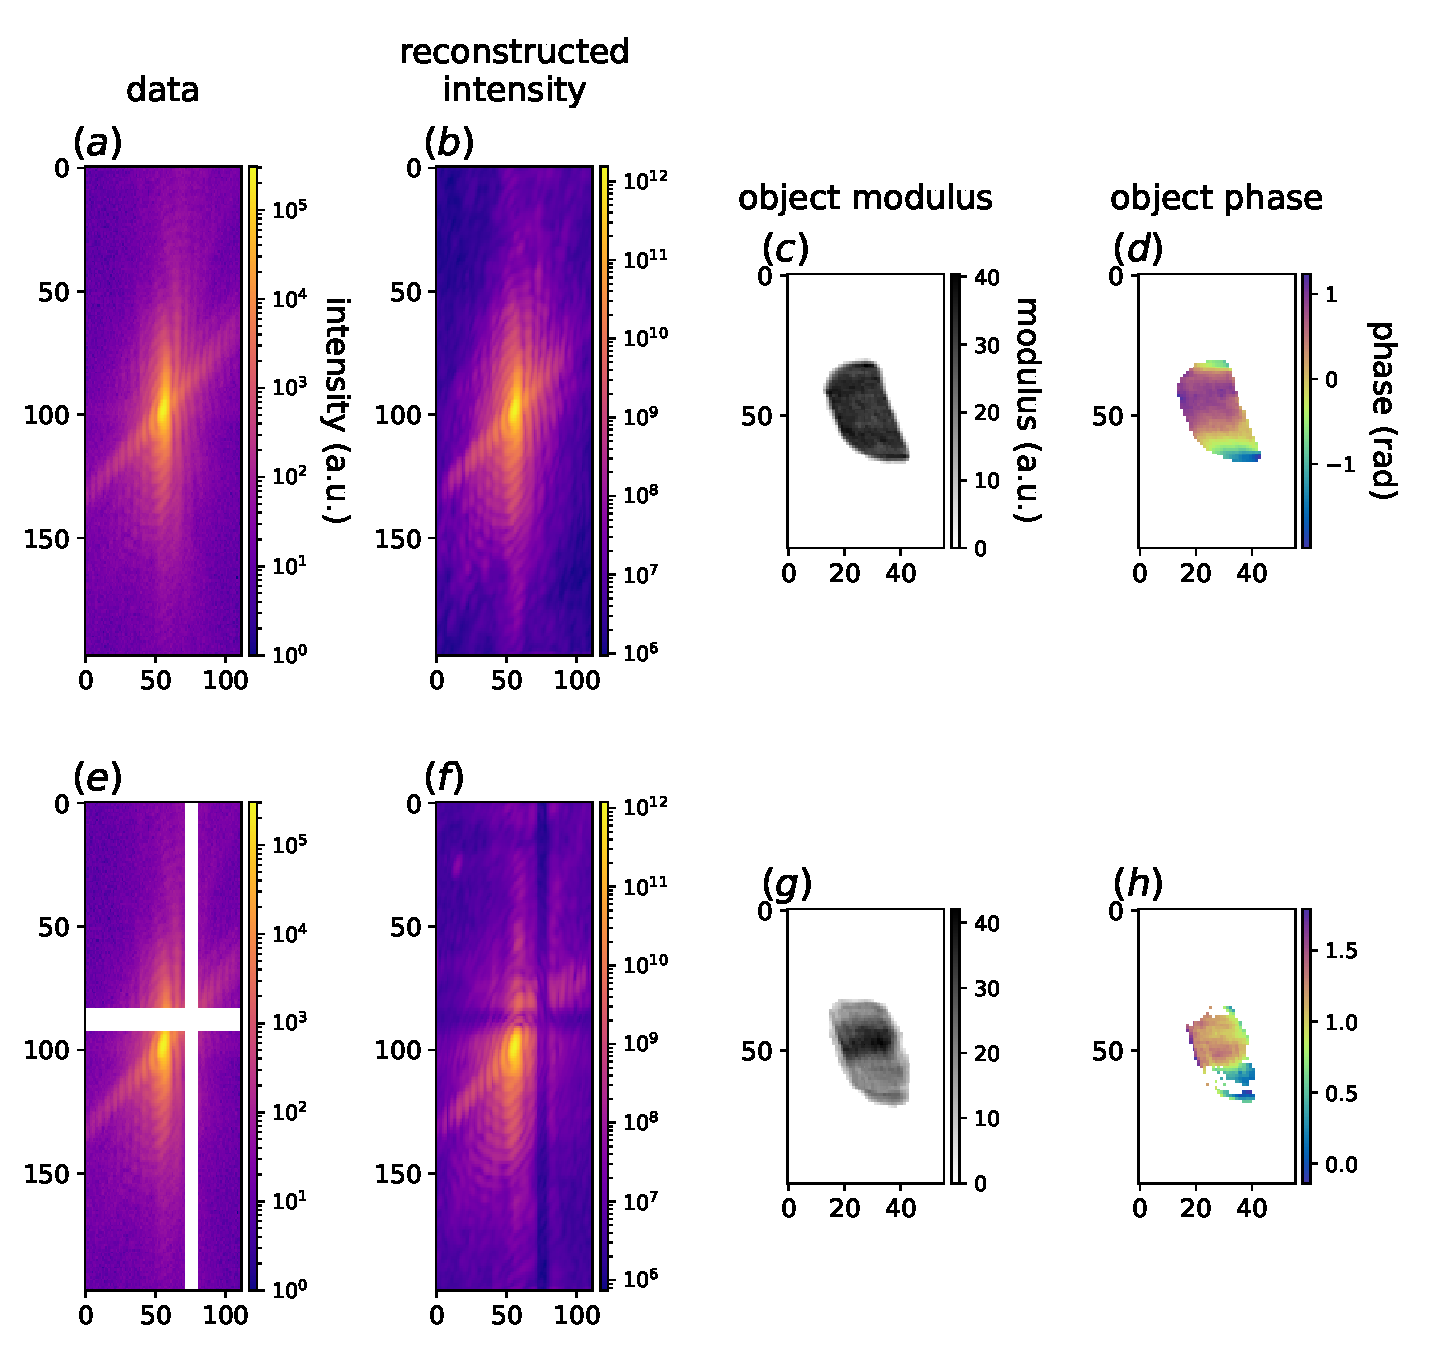
\includegraphics[width=\textwidth]{figures/Inpainting/gaps_intropdf.pdf}
    \caption{\textbf{Effect of detector gaps in BCDI reconstructions} 
    \textbf{(a)} The central xz slice of an experimental diffraction pattern. \textbf{(b)} The same slice of the diffracted
    intensity calculated from the retrieved object. \textbf{(c - d)} xz slice of the modulus and phase respectively of the particle
    obtained from the phasing of the gap-less dataset. \textbf{(e)} Same slice as in \textbf{(a)} with an artificially added
    9 pixel-wide, cross-shaped gaps to mimic the detector's ones. \textbf{(f)} The same slice of the diffracted
    intensity calculated from the retrieved object when not masking the gap regions. \textbf{(h - g)} xz slice of the modulus and phase respectively of the particle
    obtained from the phasing of the gap-affected dataset. The distortions caused by the gaps are evident. }
    \label{fig:gap_intro}
    \end{figure}


It follows that the reliability of the reconstructions in this case is 
compromised as the strain distribution can be deeply affected by the artifacts. A good practice during standard BCDI experiments
is to avoid the gaps by moving the detector if possible. However, this tends to be problematic for the case of high-resolution BCDI, 
i.e. when the diffraction pattern measurement extends to higher q-values, thus covering more than one sensing 
chip and necessarily crossing a gap region. Under these circumstances it becomes important to reduce the amount of
artifacts deriving from the gaps. 


\section{State of the art}\label{sec:InpStateArt}

Here we will discuss the current strategies employed to treat the detector gaps. As someone could argue, the simplest
yet not practical, solution would be to slightly move the detector sideways and acquire a second full scan with the
gap hiding a different region of the same Bragg peak, and then merge the two measurements into a single gap-less one. 
This would more than double the acquisition time making it, de facto, never an option during standard experiments. 

The PyNX software, routinely used for the BCDI phase retrieval at ID01, allows the user to define a mask of the gap 
regions and ignore those pixels during the execution. In this way the quality of the reconstruction improves, 
but one can still notice the presence of high-frequency oscillations appearing in both object's modulus and phase.
The origin of these artifacts can be found in the diffracted intensity calculated from the reconstructed particle as 
one can clearly see that the gap-regions is filled with nonphysically high intensity (see Fig. \ref{fig:gap_intro_mask})

\begin{figure}[h]
    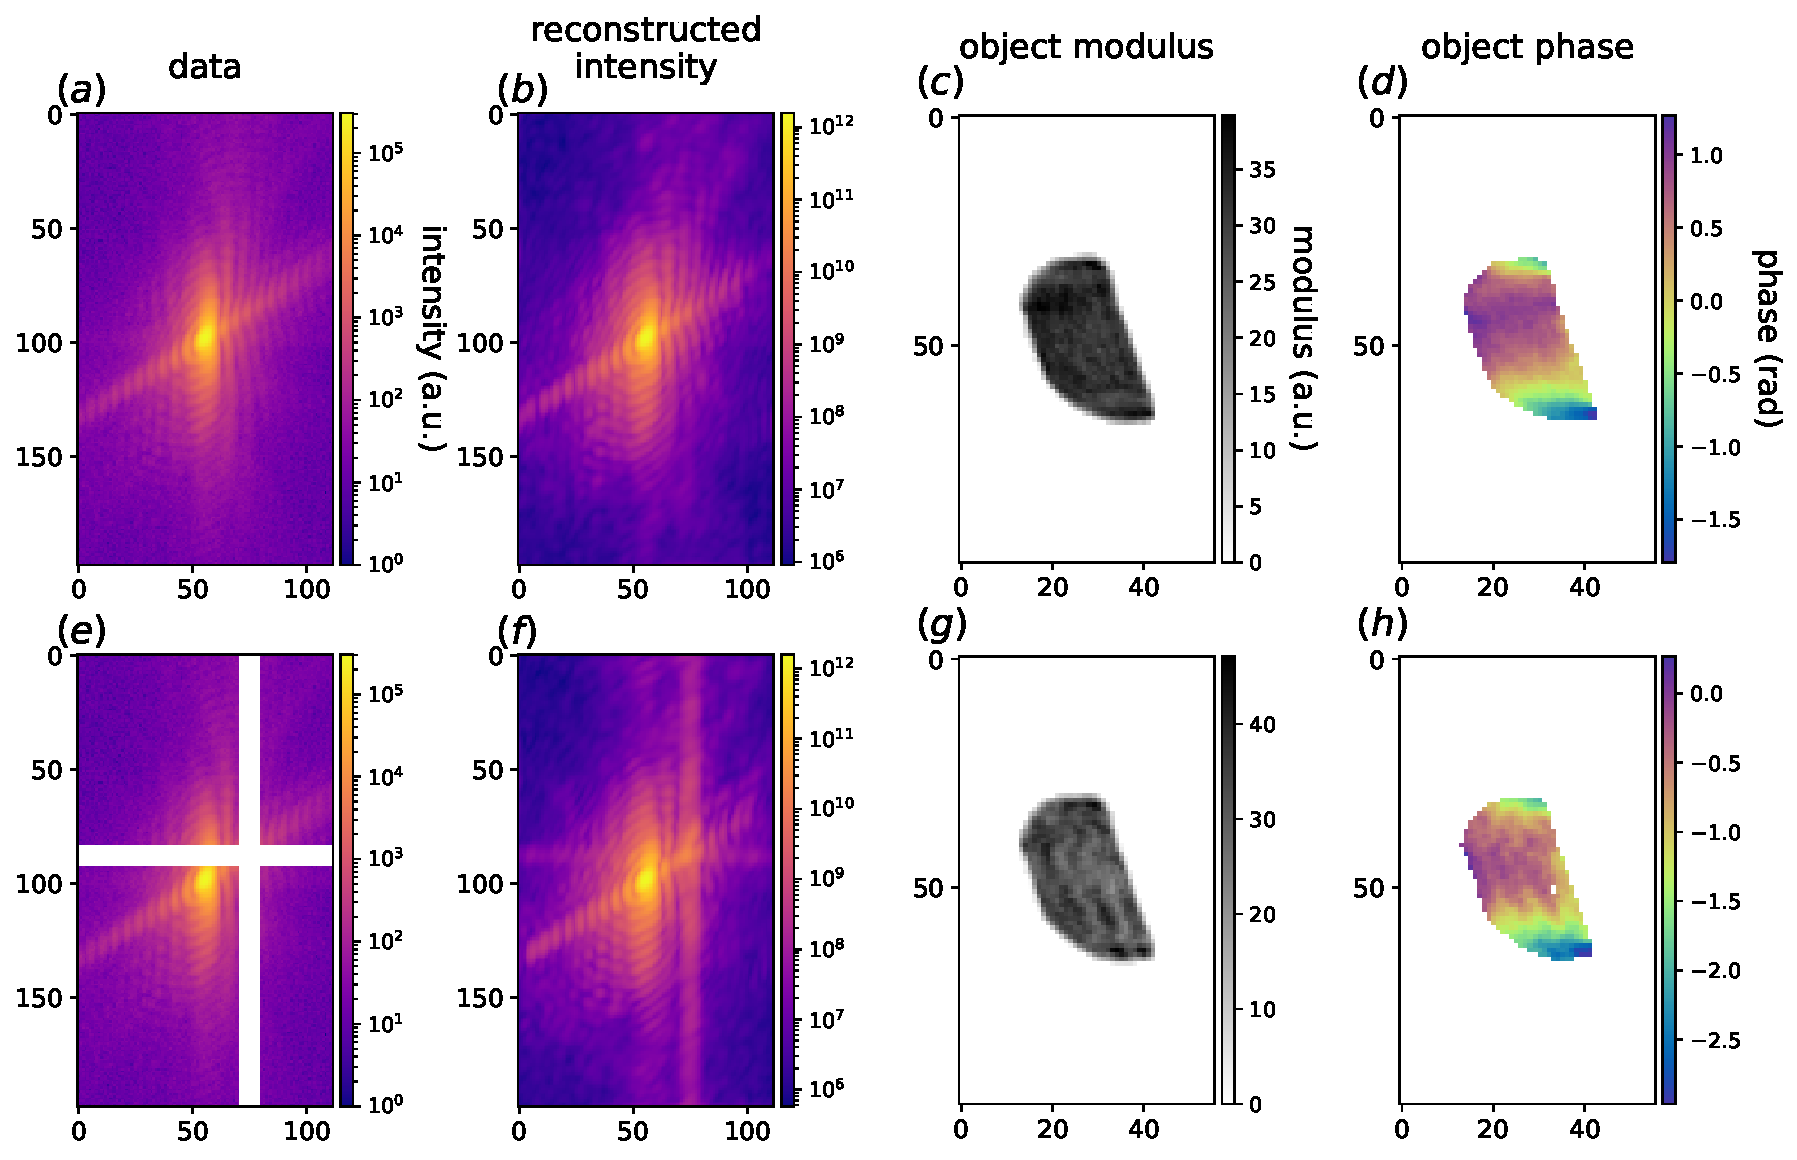
\includegraphics[width=\textwidth]{figures/Inpainting/gaps_mask.pdf}
    \caption{\textbf{Masking the gap region during phasing} 
    \textbf{(a)} The central xz slice of an experimental diffraction pattern. \textbf{(b)} The same slice of the diffracted
    intensity calculated from the retrieved object. Comparing this figure with \ref{fig:gap_intro}\textbf{(b)} one can see that
    when excluding the gap region from the phasing with a mask, the calculated intensity shows bright non-physical streaks 
    instead of the gaps. \textbf{(c - d)} xz slice of the modulus and phase respectively of the particle obtained from the 
    phasing of the gap affected data with a mask of the gap regions. Despite the much higher quality of the reconstruction, 
    one can notice some oscillatory artifacts appearing in both the modulus and the phase of the retrieved object. }
    \label{fig:gap_intro_mask}
    \end{figure}

Another, more invasive, option is to \textit{fill} these gaps with an estimate of the intensity distribution that
would be there, before the phase retrieval. These tasks of filling gap in images is usually referred to as ``inpainting''.
The following paragraph mentions the most relevant inpainting methods to give a context for our work.
    
\subsection{Background on Image Inpainting Research}

 
Computational image inpainting has been widely studied in the field of photography and imaging for many years \cite{Elharrouss_2019,reviewInpainting2021}. 
The inpainting problem can be defined as the task of utilizing known information extractable from the image, to repair
the parts where this information is missing, where for known information the colors, the textures and the semantic features
are intended. In the history of image inpainting a clear cut can be observed when deep learning methods have started to be employed.
For traditional inpainting, different techniques have been explored, from the texture synthesis methods pioneered by Efros and 
Leung \cite{Efros1999} to the use of PDEs as Navier-Stokes equations proposed by Bertalmio \textit{et al.} \cite{BertalmioNavierStokes}
and then again from sparse representations \cite{Mairal_sparse} to hybrid methods combining variational and statistical methods \cite{CedricAllene}

More recently instead, Deep Learning models, headed by Convolutional Neural Networks (CNN), have taken the place of more traditional 
methods as they can attain higher accuracy for more complex inpainting tasks. By undergoing a  
training process, CNNs can ``learn'' to recognize and reproduce the semantic features of the training dataset, and thus
leverage them during inference as additional information beside the colors and textures of the specific image to restore. 
As we have seen in \ref{ch:intro}, the typical CNN architecture for image generation consists of an encoder, which
retains the features of the input image and compresses them into a lower dimensional latent space, and a decoder, which
is responsible for the generation of the output image starting from the latent space. The model are then trained according 
to a loss function that pushes the model's predictions to be close to a given ground truth reference. 
In some cases, the loss function can be replaced by another CNN that is trained to discriminate true images from the ones
predicted by the model. These complementary networks are known as Generative Adversarial Networks (GAN), firstly 
proposed by Goodfellow \textit{et al.} \cite{goodfellow2014generativeadversarialnetworks}, and have also been used for 
image inpainting (e.g. \cite{gan_inpainting}). 
Since reviewing the vast amount of works about CNN for image inpainting is beyond the scope of this thesis and for more 
information, we redirect the reader to the reviews published by Elharrouss \textit{et al.} and Xu \textit{et al.} \cite{reviewInpainting2021,reviewInpaintingDL2023}.
as well as this blog article \cite{towardsdatascience_inpainting}. For what concerns the application of DL based 
inpainting for scientific imaging, early works date back to 2018 as in the case of Sogancioglu \textit{et al.} for x-ray 
human chest 2D radiographic images \cite{sogancioglu2018chestxrayinpaintingdeep} and to 2020 for 2D microscopic images \cite{microscopic_inpainting_2020}.
A couple of years later Tanny Chavez and coauthors published a paper comparing the performances of different CNN models 
for the inpainting of 2D x-ray diffraction images \cite{chavez_comparison_2022}. The work is precisely addressing the 
gap problem for x-ray detectors used for powder diffraction measurements and is awarding UNet and Mixed Scale Dense (MSD) 
models for the best performances on experimental data. The DL models outperform interpolations obtained with biharmonic functions
across 7 and 17 pixel-wide gaps. This work has been of inspiration for the design of our DL model for BCDI gaps inpainting.
In the same year, another work on DL based inpainting for x-ray detector gaps was published by Alfredo Bellisario 
and coauthors \cite{bellisario_noise_2022}. The authors tested a UNet-like model on the inpainting of 2D simulated, noiseless
coherent diffraction patterns against gaps of different sizes (2 to 20 pixels) along the central row. The gaps were 
placed such that the center of the peak was covered, a choice that, as we will see later, yields better results than 
predictions on peripheral areas. To our knowledge, at the time of writing, no other works about deep learning based inpainting
for X-ray detector gaps are present in the literature. \\

\section{Model design: 2D case}\label{sec:model}

On the heels of the last mentioned works we have started to tackle the detector gaps problem for BCDI using CNNs. For simplicity, we started off with 2D
case, using simulated diffraction patterns and inpainting randomly placed vertical gaps of different width. First, we created a training set of 
simulated data, composed of pairs of gap-affected images and corresponding gap-free ground truths, then built a U-Net-like model and trained it 
in a supervised fashion.

\subsection{Dataset creation}\label{sec:dataset_creation}

The creation of training datasets of simulated 2D BCDI patterns for both the gap-inpainting and phase retrieval tasks has followed the procedure
described in this paragraph.\\
In first place, once chosen the size of the array, a randomly shaped polygon is created in the center using \texttt{scipy.spatial.ConvexHull} 
function. This guarantees the object to have a compact support with homogeneous electron density as assumed for BCDI. Subsequently, 
a random phase field of the same size with variable phase range and correlation length is generated thus the complete complex object is formed.
In order to make the object more realistic a Gaussian filter and Gaussian random noise are applied to the object's modulus, so to smoothen the edges 
and simulate real cases respectively. At this point the object is resized to the shape required to match the chosen oversampling ratio and the 2D
Discrete Fourier Transform is computed. As last stage, Poisson noise is added to the diffraction patterns with different magnitudes to simulate 
various X-ray flux conditions. \\
Datasets contain a number of diffraction patterns in the order of thousands and for each of them the random variables are different as well as the 
oversampling ratios. In the datasets for the training of phase retrieval models, the reciprocal space phase corresponding to each diffraction pattern
is saved as well and used as ground truth label. 
For inpainting tasks a randomly located vertical gap mask was created and applied to the intensity data. In some cases cross-shaped gaps were 
added instead to simulate the experimental condition of the Bragg peak in the vicinity of the corner of the sensing area. 
The size of the gaps was chosen to be consistent across the dataset and four different cases were studied (3px, 6px, 9px, 12px).

\begin{figure}[h]
    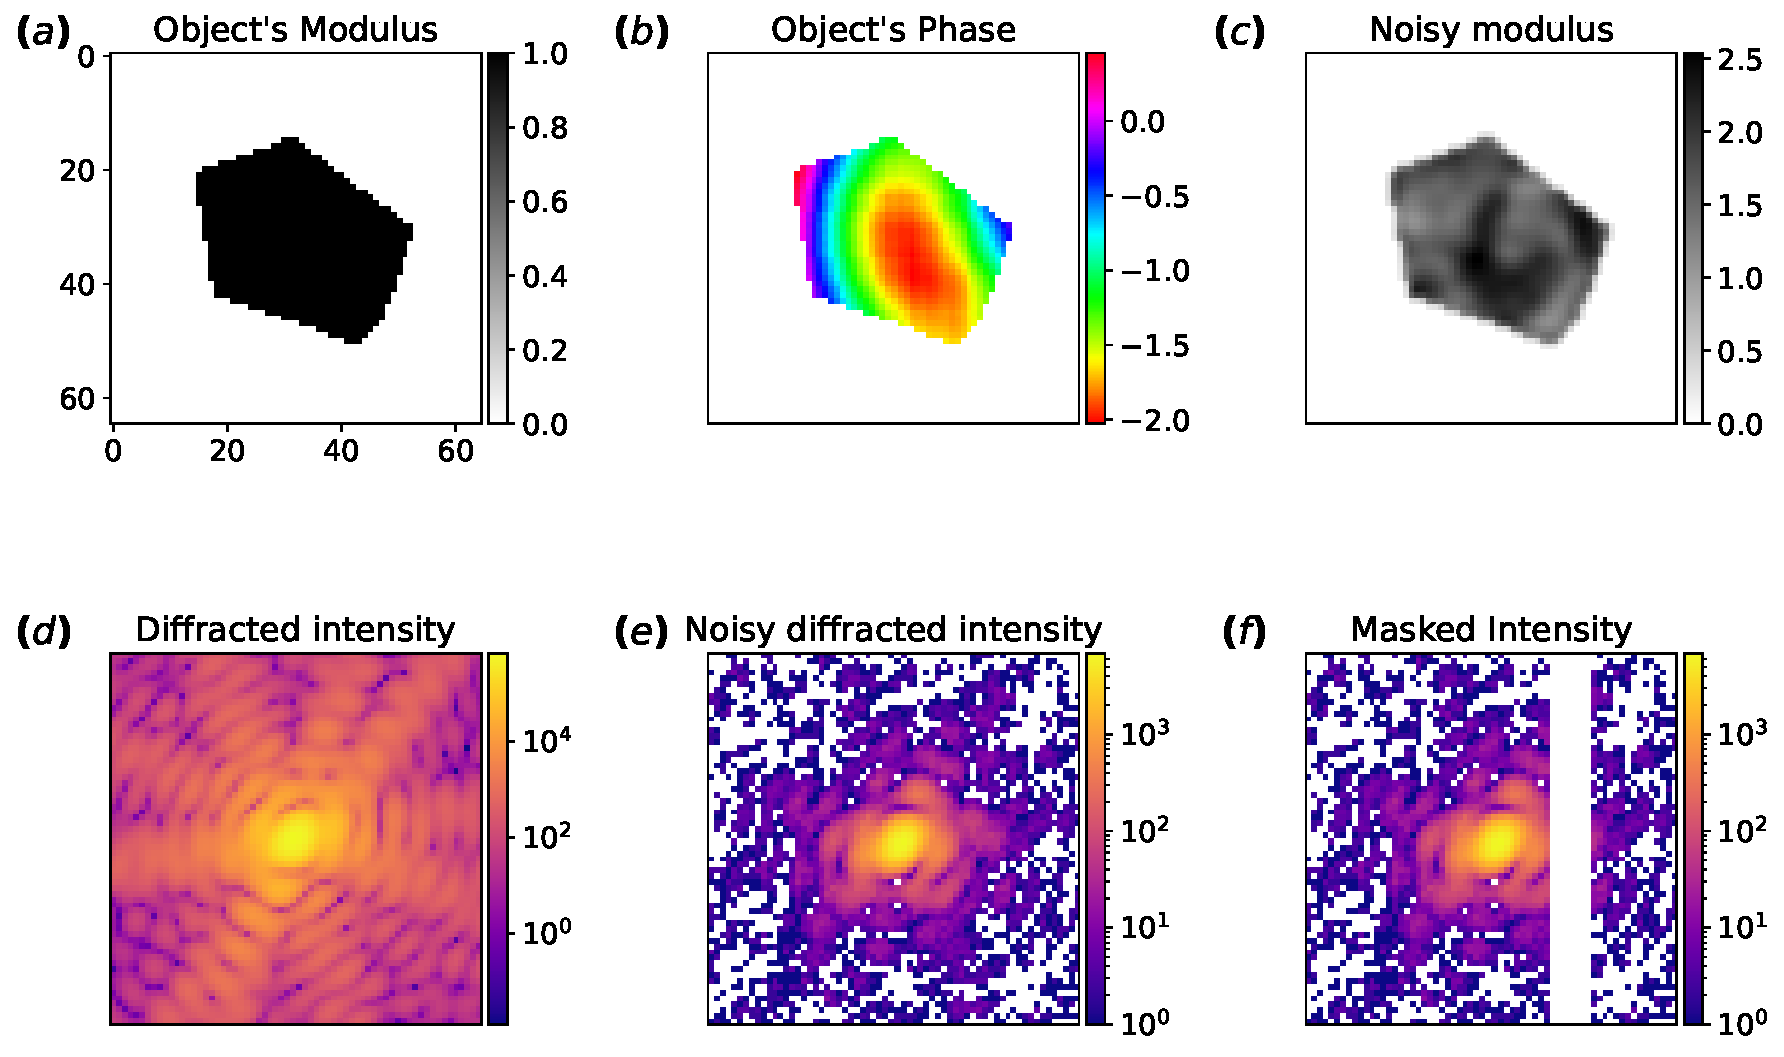
\includegraphics[width=\textwidth]{figures/Inpainting/2D_dataset_creation.pdf}
    \caption{\textbf{Steps for the simulation of a single 2D diffraction pattern} 
    \textbf{(a)} Simulated modulus of a 2D object with random shape and compact support. \textbf{(b)} Simulated object's phase
    \textbf{(c)} Object's modulus after smoothening the edges and adding random Gaussian noise. \textbf{(d)} Squared modulus of the Fourier Transform
    of the complex object (in log scale). The object is first padded with zeros to match the chosen oversampling ratio.
    \textbf{(e)} Poisson noise is added to the simulated diffracted intensity. \textbf{(f)} A 6 pixel-wide
    vertical gap is added to the diffracted intensity at a random position.}
    \label{fig:2D_dataset_creation}
\end{figure}


\subsection{2D Model design}

The 2D model that we have implemented is a U-Net that takes in input batches of 32 simulated BCDI patterns affected 
by both vertical and cross-shaped gaps. Each diffraction pattern is transformed into logarithmic scale to enhance the 
spatial features and then normalized between 0 and 1. This last passage is proven to be convenient to any DL model \cite{efficientBackProp}.
Regarding the logarithmic transformation, it is important to notice that in order to avoid problems for zero intensity
values, the $\log(I+1)$ was taken.
The shape of each image was chosen to be of $128\times128$ pixels. The inputs go through five convolutional blocks 
inside each of which a convolutional layer, a Leaky ReLU activation function and a MaxPooling operation are applied. 
The tensor's dimensionality is so reduced down to $2\times2$ while the channel dimension is brought up to 768 filters 
while the kernel size is kept at $3\times3$. In this first model we directly pass this $(32,2,2,768)$ tensor to the 
decoder that, mirroring the encoder, is composed of five blocks inside each of which there is a transposed convolutional layer
that upsamples the feature maps (stride = 2) and a Leaky ReLU activation function. We also implemented skip connections connecting each encoder block
to its corresponding shape-like decoder block. This measure has proven to be beneficial for the information flow between
encoder-decoder \cite{li_visualizing_2017}. The last activation layer of the model is a sigmoid function that guarantees an output bounded between 0 and 1 \\ 

In the first place we utilized a simple Mean Squared Error (MSE) as cost function inside the gap region only, training 
the model on 12'000 diffraction patterns over 10 epochs, with ADAM optimizer and a learning rate of $10^{-4}$. 
We have tested the Mean Absolute Error (MAE) and the Structural Similarity Index Measure (SSIM) \cite{ssim}
as well afterwards and compared the results after the same training.
Here in Fig. \ref{fig:loss_comparison} we report the comparisons for the 9 pixel-wide gap on a test simulated diffraction
pattern. The accuracy scores were calculated using the Pearson Correlation Coefficient (PCC).

\begin{equation}
    PCC = \frac{\sum_{i\in \text{gap}}(\textbf{I}_i^{\text{true}} - 
    \langle \textbf{I}^{\text{true}}\rangle)(\textbf{I}_i^{\text{pred}}-
    \langle\textbf{I}^{\text{pred}}\rangle)}{\sqrt{\sum_{i\in \text{gap}}^{}(\textbf{I}_i^{\text{true}} - 
    \langle \textbf{I}^{\text{true}}\rangle)^2}\sqrt{\sum_{i\in \text{gap}}^{}(\textbf{I}_i^{\text{pred}}-
    \langle\textbf{I}^{\text{pred}}\rangle)^2}},
        \label{eq:accuracy}
\end{equation}

Where \textbf{I} is the intensity inside the gap.

\begin{figure}[h]
    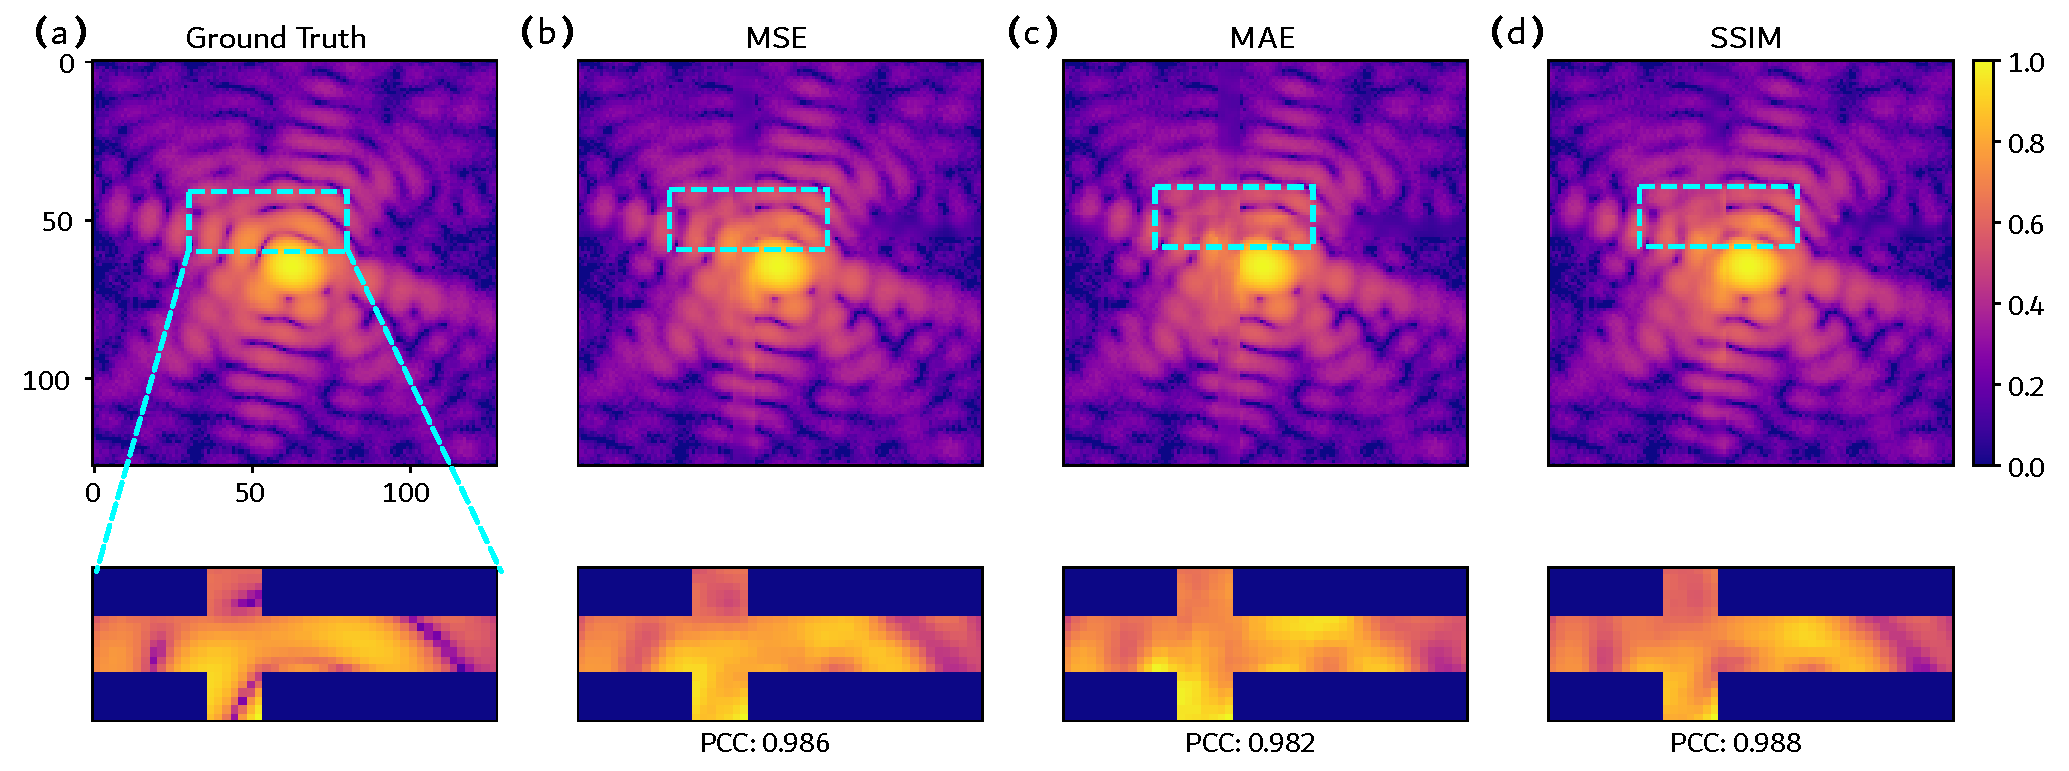
\includegraphics[width=\textwidth]{figures/Inpainting/loss_comparison.pdf}
    \caption{\textbf{Comparison of different losses} Results on a test simulated diffraction pattern for the inpainting 
    of a 9 pixel-wide cross-shaped gap produced by the same UNet model trained for 10 epochs with different loss functions. 
    \textbf{(a)} Shows the ground truth. \textbf{(b)} The prediction of the model trained with the MSE, \textbf{(c)} 
    with the MAE, \textbf{(d)} with the SSIM. Corresponding accuracy scores calculated with the Pearson Correlation 
    Coefficient (PCC) are shown as well. While MAE fails to recover the oscillations, SSIM yields better results.}
    \label{fig:loss_comparison}
\end{figure}

In the light of these results, we have decided to discard the MAE metric and adopt instead the sum of MSE and SSIM. 
At last, another term computing the MSE between the \textit{gradients} of the ground truth and predicted intensity inside
the gap region was added in the definitive loss function.\\

Once established what we considered the best loss function, we have explored different models. 
Following the work of Chavez \textit{et al.} mentioned above (\cite{chavez_comparison_2022}), we considered a 
Mixed-Scale Dense Network (MSD-Net). The advantage of this type of networks is the significant reduction of trainable
parameters, and the use of \textit{dilated} convolutions with respect to U-Net ones. While the former property guarantees
faster trainings and lower chances of overfitting, the latter enhances the capture of long-range correlations. Moreover, 
in a MSD-Net, the image's spatial dimensions are kept constant throughout the whole network as no downsampling nor upsampling is operated.
The MSD-Net that we have used consists of sequential blocks in each of which the input is transformed by two different 
convolutional layers with growing dilation rates. Each output of the convolutional layers is concatenated to the input 
feature map and the result is passed to the following block. While the kernel size is kept constant to $3\times3\times3$ pixels
the dilation rate increases linearly from 1 to 30. The last layer is a sigmoid function as well as for the U-Net. 
The total number of trainable parameters is in the order of 320'000, two orders of magnitude lower than the U-Net.
\\
In order to combine the hierarchical dimensionality reduction of the U-Net with the fine-features capturing of the MSD-Net 
we have implemented a modified U-Net that adopts dilated convolutions inside the first three encoder blocks. In particular, 
they return the input tensor concatenated with the outputs of four dilated convolutional layers computed
from the input. Dilation rates of (16,8,4,2), (10,5,3,1) and (5,3,2,1) were chosen respectively. As the MaxPooling 
operation down-samples the feature maps into smaller sizes, we limited the dilated convolutions to the first three 
blocks. Moreover, we utilized them in the encoder layers only as they are mostly used for feature extraction \cite{dilated_conv}.
The characteristics of each model are summarized in form of pseudo - code in Table \ref{tab:model_comparison}.
\\

The three different models have been trained with a combined loss function (MSE + SSIM + MSE on the gradients ) on the 
same training dataset for 10 epochs each.  The results showed poor performances of the MSD-Net with respect to the two 
U-Nets. Slightly higher accuracy was achieved by our modified U-Net. 

\begin{figure}[h]
    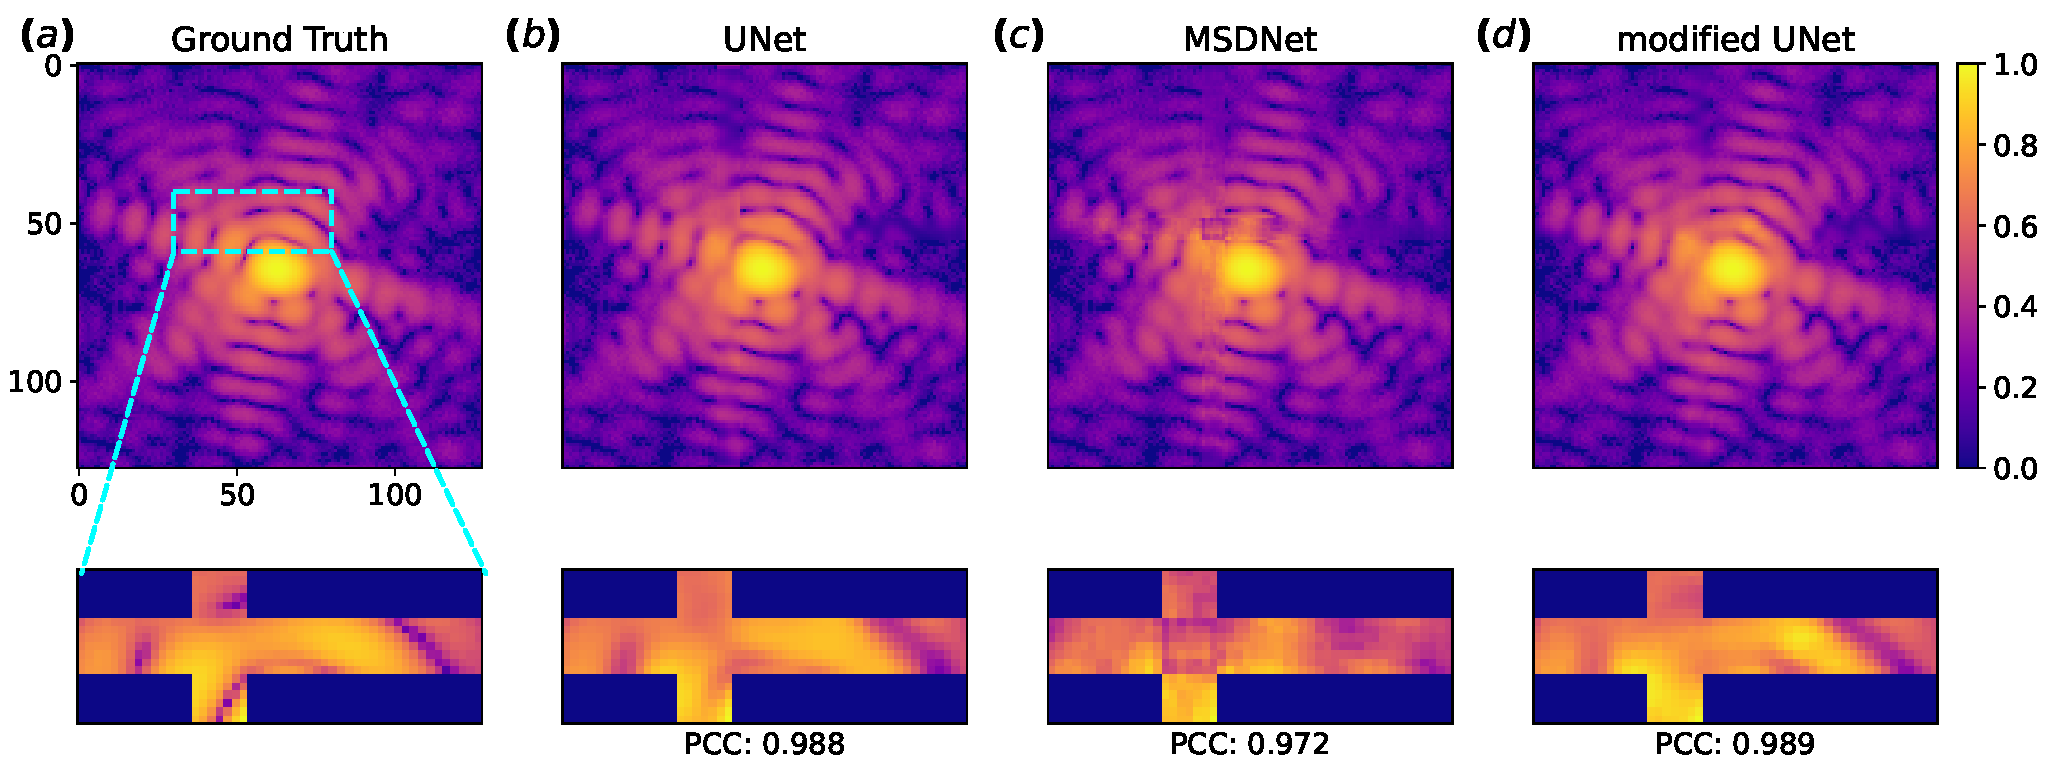
\includegraphics[width=\textwidth]{figures/Inpainting/model_comparison.pdf}
    \caption{\textbf{Comparison of different models} Results on a test simulated diffraction pattern for the inpainting 
    of a 9 pixel-wide cross-shaped gap using three different models trained with the same loss function.
    \textbf{(a)} Shows the ground truth. \textbf{(b)} The prediction of the U-Net, \textbf{(c)} 
     of the MSD-Net, \textbf{(d)} of the modified U-Net. Corresponding accuracy scores calculated with the Pearson Correlation 
    Coefficient (PCC) are shown as well.}
    \label{fig:models_comparison}
\end{figure}


\begin{table}[h!]
    % \small 
    %  or 
    \scriptsize
    \centering
    % \resizebox{\textwidth}{!}{%
    \begin{tabular}{|>{\centering\arraybackslash\bfseries}p{1.2cm}|p{4.5cm}|p{4.5cm}|p{4.5cm}|}
    \hline
     & \textbf{U-Net} & \textbf{MSD-Net} & \textbf{Unet\_mod} \\ \hline
    block1 & 
    \begin{lstlisting}[basicstyle=\tiny\ttfamily, xleftmargin=-1em]
    def encoder_block(x_input, num_filters, ker):
        s = Conv2D(num_filters, ker,'leaky_relu')(x_input)
        x = MaxPool2D(2)(s)
        return x, s
    \end{lstlisting} 
    & \begin{lstlisting}[basicstyle=\tiny\ttfamily, xleftmargin=-1em]
    def MSD_block(x, in_channels, dilations,kernel_size=3):  
        if isinstance(dilations, int):  
            dilations = [(j % 10) + 1 for j in range(dilations)]  
        out_channels = in_channels + len(dilations)  
        for d in dilations:  
            x1 = Conv2D(out_channels//2,kernel_size,1, dilation_rate=dilation, 'same', 'leaky_relu')(x)
            x = tf.concat([x1,x] ,axis = -1)
        return x, out_channels
    \end{lstlisting} 
    &
    \begin{lstlisting}[basicstyle=\tiny\ttfamily, xleftmargin=-1em]
    def encoder_block_mod(x_input, ker, num_filters, rate):
        f = num_filters // 4
        s = tf.concat([x_input] + [Conv2D(f, ker, dilation_rate=r, 'leaky_relu')(x_input) for r in rate], axis=-1)
        return MaxPool2D(2)(s), s
    \end{lstlisting} \\ \hline
    block2 
    &
    \begin{lstlisting}[basicstyle=\tiny\ttfamily, xleftmargin=-1em]
    def decoder_block(x_input, num_filters, ker, skip_input = None):
    
        if skip_input is not None:
            x_input = Concatenate()([x_input, skip_input])
            
        x = Conv2DTranspose(num_filters, ker, strides=2, 'leaky_relu')(x_input)
        return x
    \end{lstlisting} 
    & 
    &
    \begin{lstlisting}[basicstyle=\tiny\ttfamily, xleftmargin=-1em]
    def decoder_block(x_input, num_filters, ker, skip_input = None):
    
        if skip_input is not None:
            x_input = Concatenate()([x_input, skip_input])
            
        x = Conv2DTranspose(num_filters, ker, strides=2, 'leaky_relu')(x_input)
        return x
    \end{lstlisting} \\ \hline
    
    body & 
    \begin{lstlisting}[basicstyle=\tiny\ttfamily, xleftmargin=-1em]
        x, s1 = encoder_block(inputs, 48,3)        
        x, s2 = encoder_block(x, 96,3)             
        x, s3 = encoder_block(x, 192,3)           
        x, s4 = encoder_block(x, 384,3)           
        x, s5 = encoder_block(x, 768,3)          
    
        x = Conv2D(1536,3, 'leaky_relu')(x) 
    
        x = decoder_block(x,768,3)
        x = decoder_block(x,384,3, s5)
        x = decoder_block(x, 192,3,s4)
        x = decoder_block(x, 96,3,s3)
        x = decoder_block(x, 48,3,s2)
        
        x = Conv2D(24,5,'leaky_relu')(x) 
        x = Conv2D(12,5,'leaky_relu')(x)
        x = Conv2D(6,5,'leaky_relu')(x)
        
        out = Conv2D(1,5,'sigmoid')(x)
    \end{lstlisting} 
    & 
    \begin{lstlisting}[basicstyle=\tiny\ttfamily, xleftmargin=-1em]
        x,out_ch = MSD_block(inputs,1,[1,2])
        x,out_ch = MSD_block(x,out_ch,[3,4])
        ...
        ...
        x,out_ch = MSD_block(x,out_ch,[31,32])
        out = Conv2D(1,3,'sigmoid')(x)
    \end{lstlisting} 
    &
    \begin{lstlisting}[basicstyle=\tiny\ttfamily, xleftmargin=-1em]
        x, s1 = encoder_block_mod(inputs,3,48,[16,8,4,2])   
        x, s2 = encoder_block_mod(x,3, 96,[10,5,3,1])       
        x, s3 = encoder_block_mod(x,3, 192,[5,3,2,1])           
        x, s4 = encoder_block(x, 384 ,3)            
        x, s5 = encoder_block(x, 768, 3)                    
        
        x = Conv2D(1536,3,'leaky_relu')(x)
        
        x = decoder_block(x,768,3)    
        x = decoder_block(x,384,3,s5)  
        x = decoder_block(x,192,3,s4)  
        x = decoder_block(x,96,3,s3) 
        x = decoder_block(x,48,4,s2)  
    
        x = Concatenate()([x, s1])
        x = Conv2D(24,5,'leaky_relu')(x) 
        x = Conv2D(12,5,'leaky_relu')(x)   
        x = Conv2D(6,5,'leaky_relu')(x)
    
        out = Conv2D(1,3,'sigmoid')(x)
    \end{lstlisting} \\ \hline
    parameters & 31,827,673 & 322,458 & 32,652,337 \\ \hline
    \end{tabular}
    \caption{Comparison of Unet, MSDNet, and Unet\_mod components.}
    \label{tab:model_comparison}
\end{table}

We conclude here the introductory studies on 2D simulated data. These preliminary tests served to get familiar with 
the different DL architectures and loss functions and select the optimal choices for the inpainting of BCDI detector
gaps. 

\subsection{Accuracy VS Gap position}

Before moving to the 3D case, it is worth spending a few words on the assessment of the DL model upon different conditions.
We leave the assessment of the prediction accuracies against the gap size for the 3D case and will focus instead on two
other evaluations. Namely, the accuracy as function of the position of the gap inside the diffraction pattern and the 
as a function of the oversampling ratio.
For the first test we have simulated 150 2D diffraction patterns from random particles shapes, random oversampling ratios
and Poisson noise intensity. For each diffraction pattern we have then placed a vertical 9 pixel-wide gap at all positions
from left to right, computed the DL prediction and corresponding accuracy score when compared to the ground truth. The 
accuracy was again calculated with the Pearson Correlation Coefficient. We have then averaged this score for each 
gap position, over the 150 diffraction patterns and plotted the result as a function of the gap position. Fig. \ref{fig:accVSpos} 
shows the resulting curve that clearly highlights that the model performs better regions with high intensity. 
This can be qualitatively explained with different reasons: (i) central regions have larger features both because of the 
nature of the Bragg peak, and because of the lower noise level. This makes it easier for the model as it reduces the 
complexity of the prediction. (ii) As we move away from the center of the Bragg peak, the Signal to Noise Ratio (SNR) 
decreases, along with the \textit{density of signal}. High accuracy scores in these regions would require the model to be 
able to predict noise correctly which is by definition impossible as it is an uncorrelated random process. One could argue 
that the accuracy curve would follow the statistical distribution of the gap positions inside the DL model training dataset.
However, each mask has been applied at a position drawn from a discrete uniform probability function spanning in the full
data size, thus we exclude this hypothesis. 

\begin{figure}[h]
    \centering
    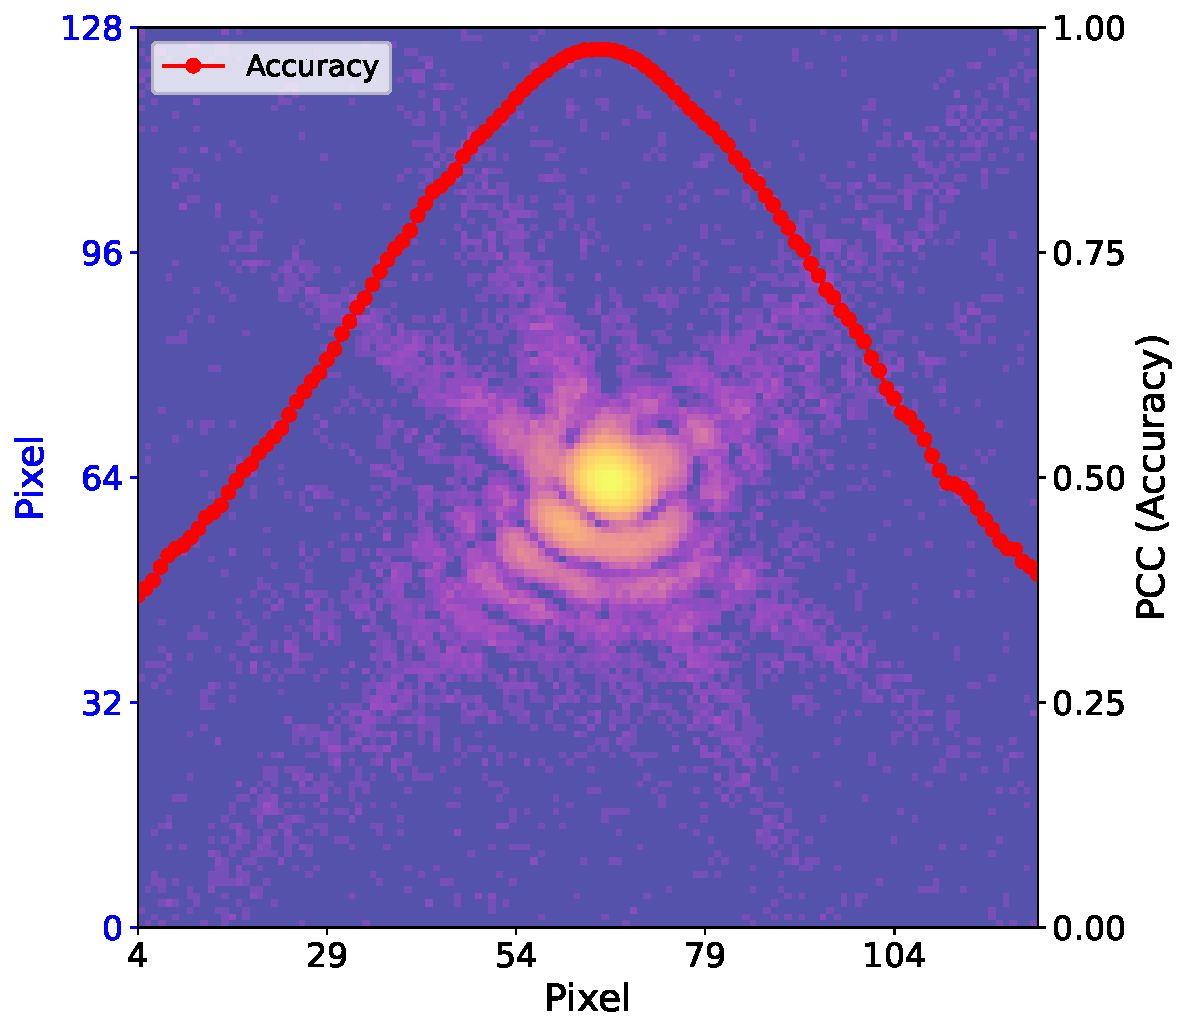
\includegraphics[width=.7\textwidth]{figures/Inpainting/2D_acc_pos.pdf}
    \caption{\textbf{(Accuracy VS Gap position)} Average Pearson Correlation Coefficient calculated over 150 
    9 pixel-wide vertical predicted gaps for each position of the gap inside the diffraction patterns. The model 
    shows higher accuracies for high intensity regions.}
    \label{fig:accVSpos}
\end{figure}

To conduct the second test, we simulated 150 diffraction patterns for the same particle varying gradually the oversampling
ratio between 2 and 6. For each image we have then applied a 9 pixel-wide vertical gap at all $X$ positions and performed 
the DL prediction. The accuracy scores have been averaged for each prediction in the same image and plotted against the oversampling 
(Fig. \ref{fig:accVSovs}). As expected from the above considerations, the model performs better for larger oversampling ratios, 
because of the bigger size of the features with respect to the gap width and because of the more uniform \textit{density of signal}.
About this last concept, it is worth clarifying that, for a given particle, the total amount of intensity in the
diffraction patterns is in principle constant regardless of the oversampling ratio as it is fixed by Parseval theorem.
However, if the size of the dataset is kept fixed for different oversamplings, the effect is the same of a zoom lens
that increases or reduces the field of view. Therefore, while for low oversampling ratios the full peak is recorded, 
for higher ones the peak is cropped, and less intensity is present in the image. This effect, coupled with the typical radial
intensity decay of Bragg peaks and the presence of Poisson noise, makes largely oversampled BCDI patterns having a smaller
and more uniform \textit{density of signal}, intended as the amount of information per pixel. On the contrary, for low 
oversampling ratio the \textit{density of signal} is less uniform as it is high inside bright regions (lot of information
concentrated in few pixels) and low in noisy regions far from the peak. It follows that in order to properly assess the accuracy
against the oversampling ratio one should consider diffraction patterns over the same extent in Q-space, thus changing 
the size of the images. This more accurate evaluation was carried out for the 3D case and can be found in the next section.

\begin{figure}[h]
    \centering
    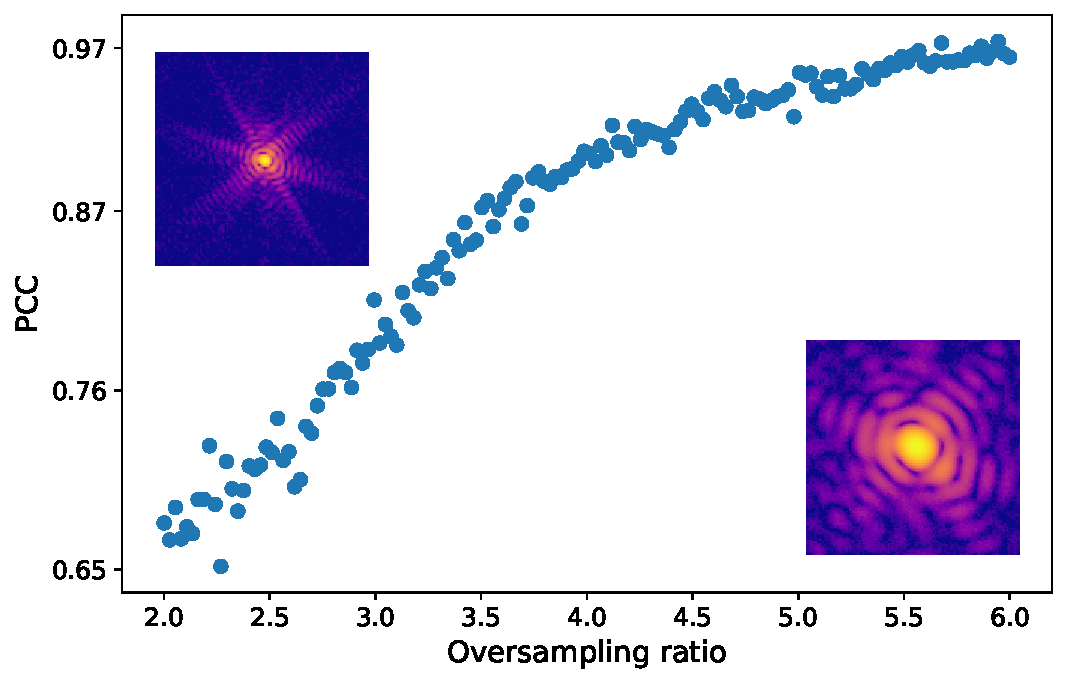
\includegraphics[width=.7\textwidth]{figures/Inpainting/2D_acc_ovs.pdf}
    \caption{\textbf{(Accuracy VS Oversampling ratio)} Average Pearson Correlation Coefficient calculated over 280
    9 pixel-wide vertical predicted gaps for each position of the gap inside the diffraction patterns. The model 
    shows higher accuracies for high intensity regions.}
    \label{fig:accVSovs}
\end{figure}

\section{3D case - Patching approach}\label{sec:patching}

When considering the 3D case, and especially the experimental conditions, there are a few practical issues that needs
to be overcome. In fact, experimental BCDI datasets that are more often affected by detector's gaps are necessarily large
datasets (e.g. $512 \times 512 \times N_{\text{rocking\_steps}}$). Training a U-Net like model for 3D images of that size is 
overly expensive in terms of computing memory and time. Moreover, a common problem with this type of architectures is that
the size of the images they can process is fixed by the first initialization. This means that one would need to resize, via 
binning or interpolation, the experimental datasets to the shape accepted by the DL model, and back to the original
shape after the inpainting. Besides the impracticality, these operations are not recommended as they induce further
modification and information loss to the original data. For these reasons we have opted for a patching approach that 
loosens these constraints while preserving sufficiently high accuracies. \\

The patching method exploits the regularity of the oscillations within BCDI datasets. The periodicity of the fringes 
in reciprocal space, peculiar property of this coherent diffraction technique, can be observed by eye and in many cases 
makes the prediction inside a gap region intuitively possible starting from just a few neighboring pixels. 
In our case we have decided to work with 32 pixel-sided cubic sub-volumes (patches from now on) cropped out of entire diffraction 
patterns. Among the ``GPU-friendly'' tensor sizes \cite{nvidia_tensor_cores_optimization} we opted for 32 as good trade-off
between amount of contained information and computing power required for training and inference. 

\subsection{Dataset creation}
The training dataset consists of 50\% patches from experimental data and 50\% from simulated data.
The experimental measurements were acquired at the ID01 beamline of the ESRF during different beamtimes on different particles.
Namely, (i) Pt particles dewetted on sapphire and YSZ (yttria–stabilized zirconia) with Winterbottom shape, 
measured under various temperatures and gas conditions, (ii) Pd and PdCe particles on glassy carbon, with
Wulff shape, measured in an electrochemical environment following hydrogen loading. (iii) Ni particles on sapphire undergoing
changes during $CO_2$ adsorption and (iv) cubic $CaCO_3$ particles on glassy carbon.
\\
The synthetic diffraction patterns were instead simulated in three steps. The first step consisted in the creation of 
simulated 3D particles of different shapes (Winterbottom, Wulff, Cubic, Octahedral and random) using pre-existing scripts
developed by Dr. Dupraz and Dr. Bellec \cite{lim_convolutional_2021}. These codes allow the user to construct a cubic FCC
crystal of a given element, taking into account the inter-atomic potential, the atomic mass
and the lattice parameter. The final particle is finally obtained by "cutting" off atomic planes along given (or random)
directions, depending on the chosen shape. We have simulated only Gold nano-particles and this is, in first approximation,
equivalent to any generic element as a different lattice parameter would just shift the Bragg peak to a different 
position in reciprocal space, with no significant alterations of the diffraction pattern.  
Each particle's configuration is then automatically saved in a LAMMPS-readable file. In a second stage, we perform 
energy relaxation using LAMMPS software for Molecular Dynamics. This step induces small displacements to the perfect 
lattice, especially near the surface. In the last stage, the 3D diffraction pattern of a selected Bragg 
reflection is computed using PyNX scattering package \cite{pynx_scattering}. This software, optimized for GPU 
acceleration, produces a 3D representation of a selected Bragg peak. 
It is then possible to adjust the parameters that control the oversampling ratio, the size of the array in which the 
Bragg peak is centered and the rotation of the Q-space. In our case we simulated 128 pixel-size cubic diffraction 
patterns and, in order to augment the training dataset, we did it for various oversampling ratios (from 2 to 5) and 
different rotations for each particle. As we have seen in Chapter (ref to introduction), in the kinematic scattering 
approximation the energy of the incident X-ray does not alter the diffraction pattern if not as a "zooming" factor. 
Thus, in our case we don't need to explicitly account for different energies as we already vary the oversampling ratio. 
Before taking portions of these simulated BCDI patterns, we added Poisson noise randomly scaling the $\lambda$ parameter
for each image.


\begin{figure}[h]
    \centering
    \begin{subfigure}{0.45\textwidth} % Adjust width as needed
        \centering
        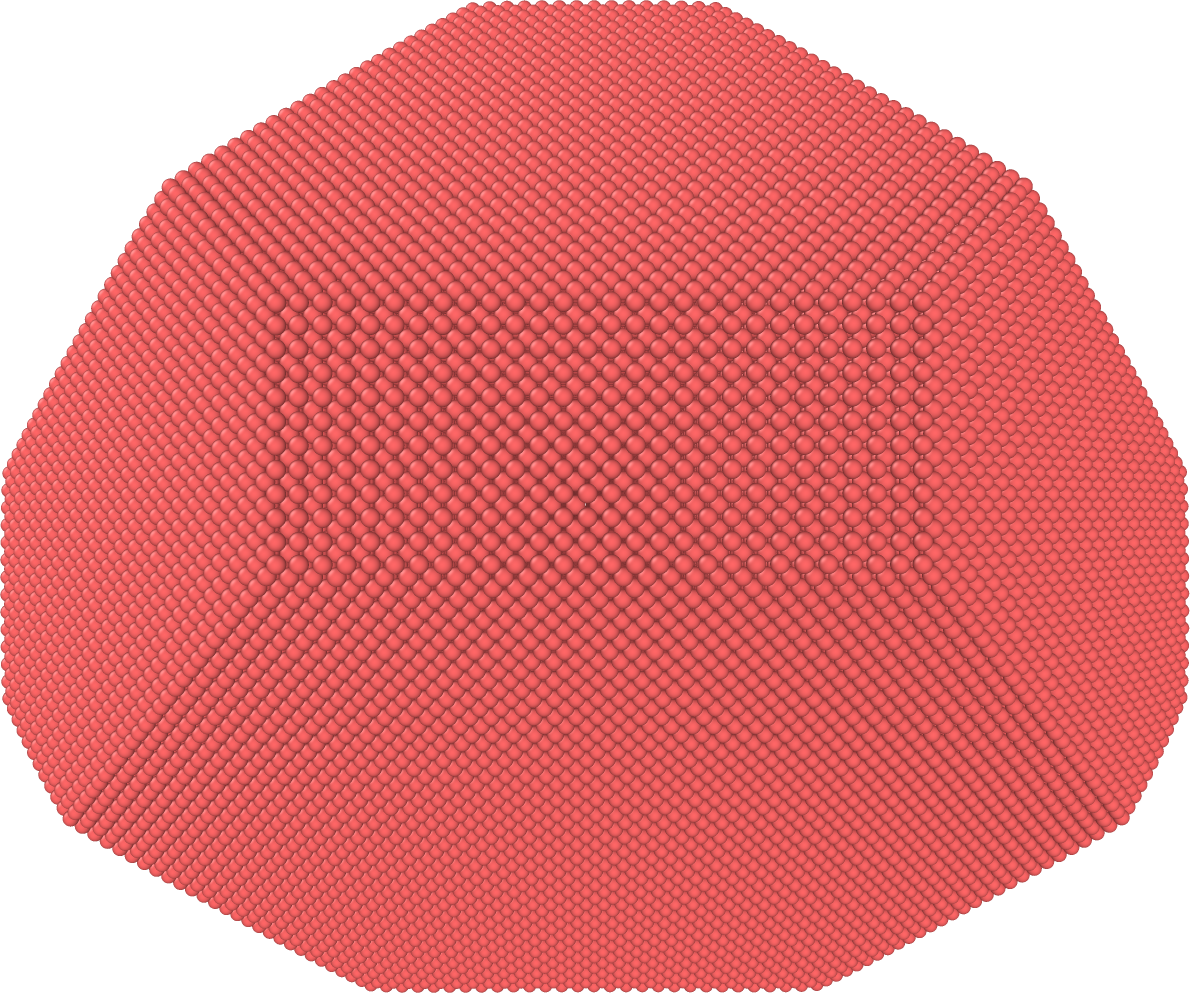
\includegraphics[width=\linewidth]{figures/Inpainting/crystal.png}
        \caption{\textbf{(a)}}
    \end{subfigure}
    \hfill
    \begin{subfigure}{0.45\textwidth}
        \centering
        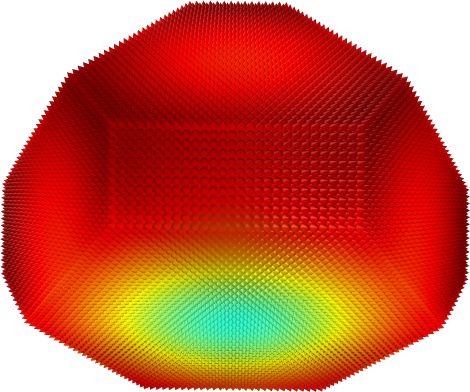
\includegraphics[width=\linewidth]{figures/Inpainting/displacement_field.png}
        \caption{\textbf{(b)}}
    \end{subfigure}
    \caption{\textbf{(a)} Simulated Au particle with Winterbottom shape (134114 atoms).\textbf{(b)} Atomic 
    displacement field of the same particle after LAMMPS energy relaxation. 
    It is evident the typical distribution at the interface with the substrate.}
    \label{fig:comparison}
\end{figure}


At this point, we proceeded with the extraction of sub-volumes taken at \textit{pseudo}-random locations inside each 3D pattern. 
The selection in fact was not totally random as we favored the extraction of sub-volumes from the outer regions, far from the 
center of the peak. There are mainly two reasons for this choice, namely (i) compensate the inherent uneven accuracy score against
the position of the gap (see Fig.\ref{fig:accVSpos}) by increasing the training data far from the center and (ii) emulate
as much as possible the experimental conditions, in which unavoidable gaps are typically far from the center of the peak.
For each sub-volume a 3D mask of the gap was created for different gap sizes (3,6,9,12 pixel-wide). The gap was placed 
vertically, in the center, along the third dimension, resulting in a ``empty slab''. Cross-shaped gaps were also 
included in the training dataset, with a population ratio of 1:5 compared to vertical gaps. They were created by 
adding a horizontal gap at a random height to an existing vertical gap.
The final training dataset consisted of 30'000 $32\times32\times32$ sub-volumes created as described above. 

\begin{figure}[h]
    \centering
    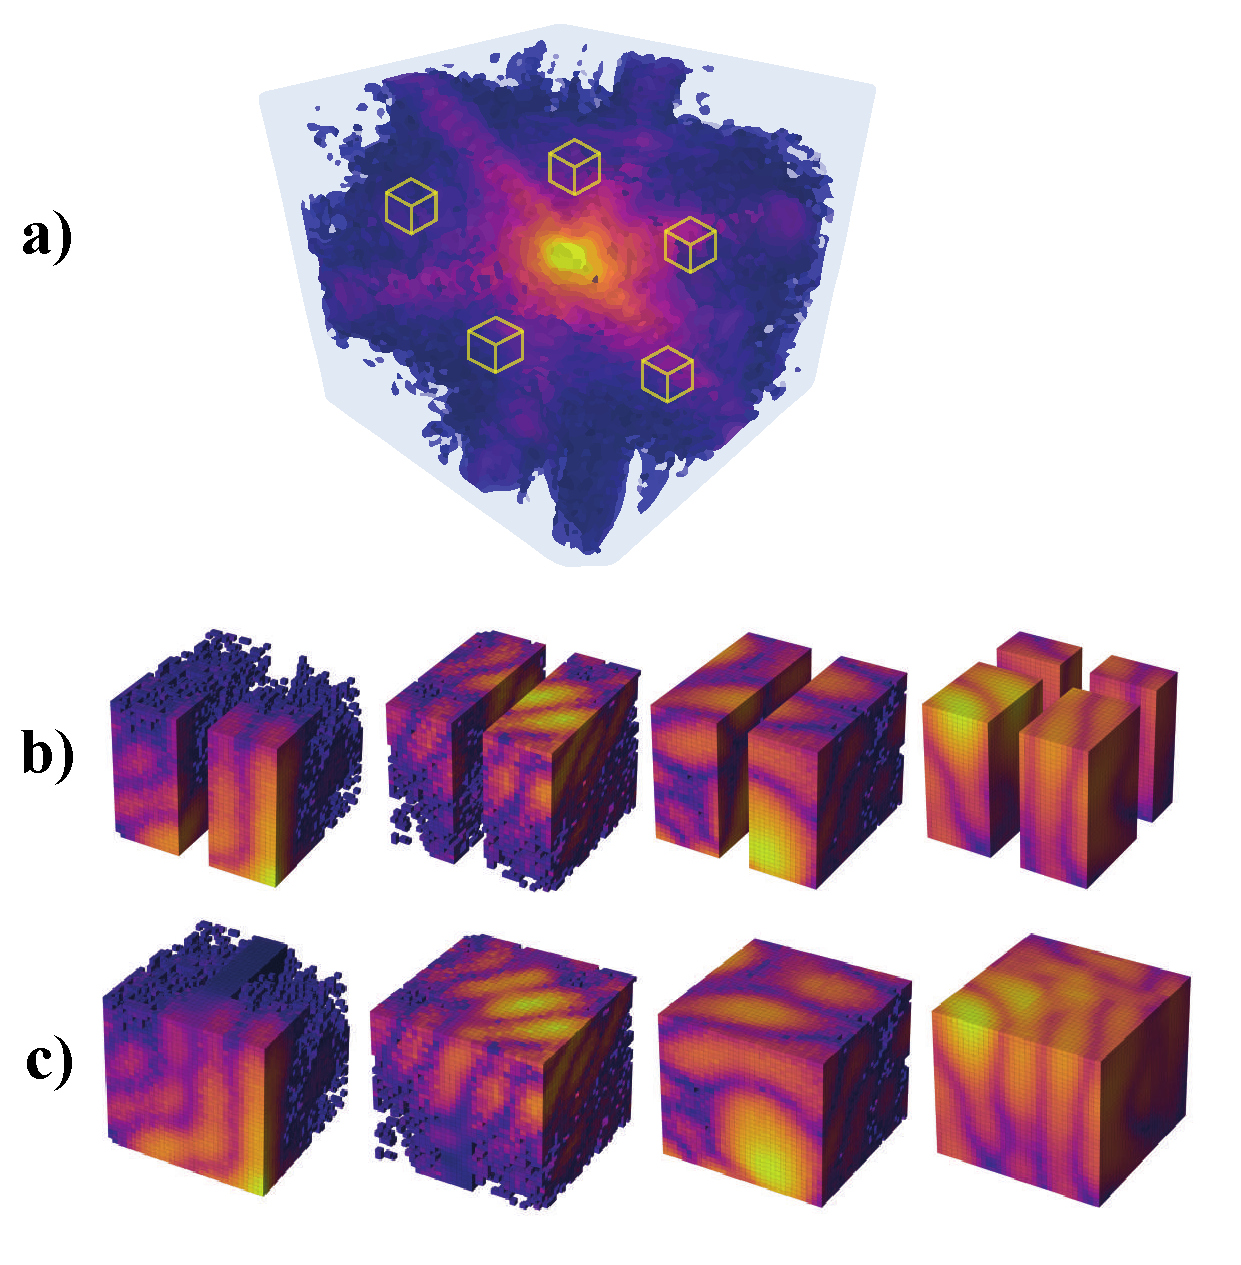
\includegraphics[width=.6\textwidth]{figures/Inpainting/process.pdf}
    \caption{\textbf{Schematic of the sub-volumes extraction.} \textbf{a)} The 3D BCDI diffraction pattern and the 
    sub-volumes. \textbf{b)} $32\times32\times32$ pixel-size sub-volumes with 9 pixel-wide vertical and cross-shaped gaps.
    \textbf{c)} Same sub-volumes with the DL inpainted gaps.}
    \label{fig:architecture3d}
\end{figure}

\section{3D model architecture}

The DL architecture used for the 3D patching inpainting is illustrated in Fig. \ref{fig:architecture3d}.  
Given the reduced size of the inputs, the encoder this time is composed of four blocks only, in each of which there
are convolutional layers and max pooling layers. The feature map is thus reduced to a $2\times2\times2\times478$ tensor 
before being passed to the decoder. Notice that, as introduced above in section Sec.\ref{sec:model}, we have employed
dilated convolutions in the first two blocks to enhance the extraction long-range correlated features. After four decoder
blocks we have put three simple convolutional layers with 24,12 and 6 channels respectively, in order to restore the possible
smoothing effect of the decoder. Same as in the 2D model, the last activation function is a sigmoid that ensures the output
to be in the range (0,1). 
The model contains 2'770'000 trainable parameters, significantly less than the 2D models working on full size patterns. 
\\
The training was performed loading batches of 32 images at the time over 100 epochs using ADAM optimizer \cite{ADAM}. 
We initialized the optimizer with a learning rate of $10^{-3}$ and decreased it progressively with the 
\texttt{ReduceLROn-Plateau} callback feature available in Tensorflow. In order to exploit at maximum the training 
dataset we left only 4\% and 2.5\% of the whole dataset for validation and testing respectively.  

\begin{figure}[h]
    \centering
    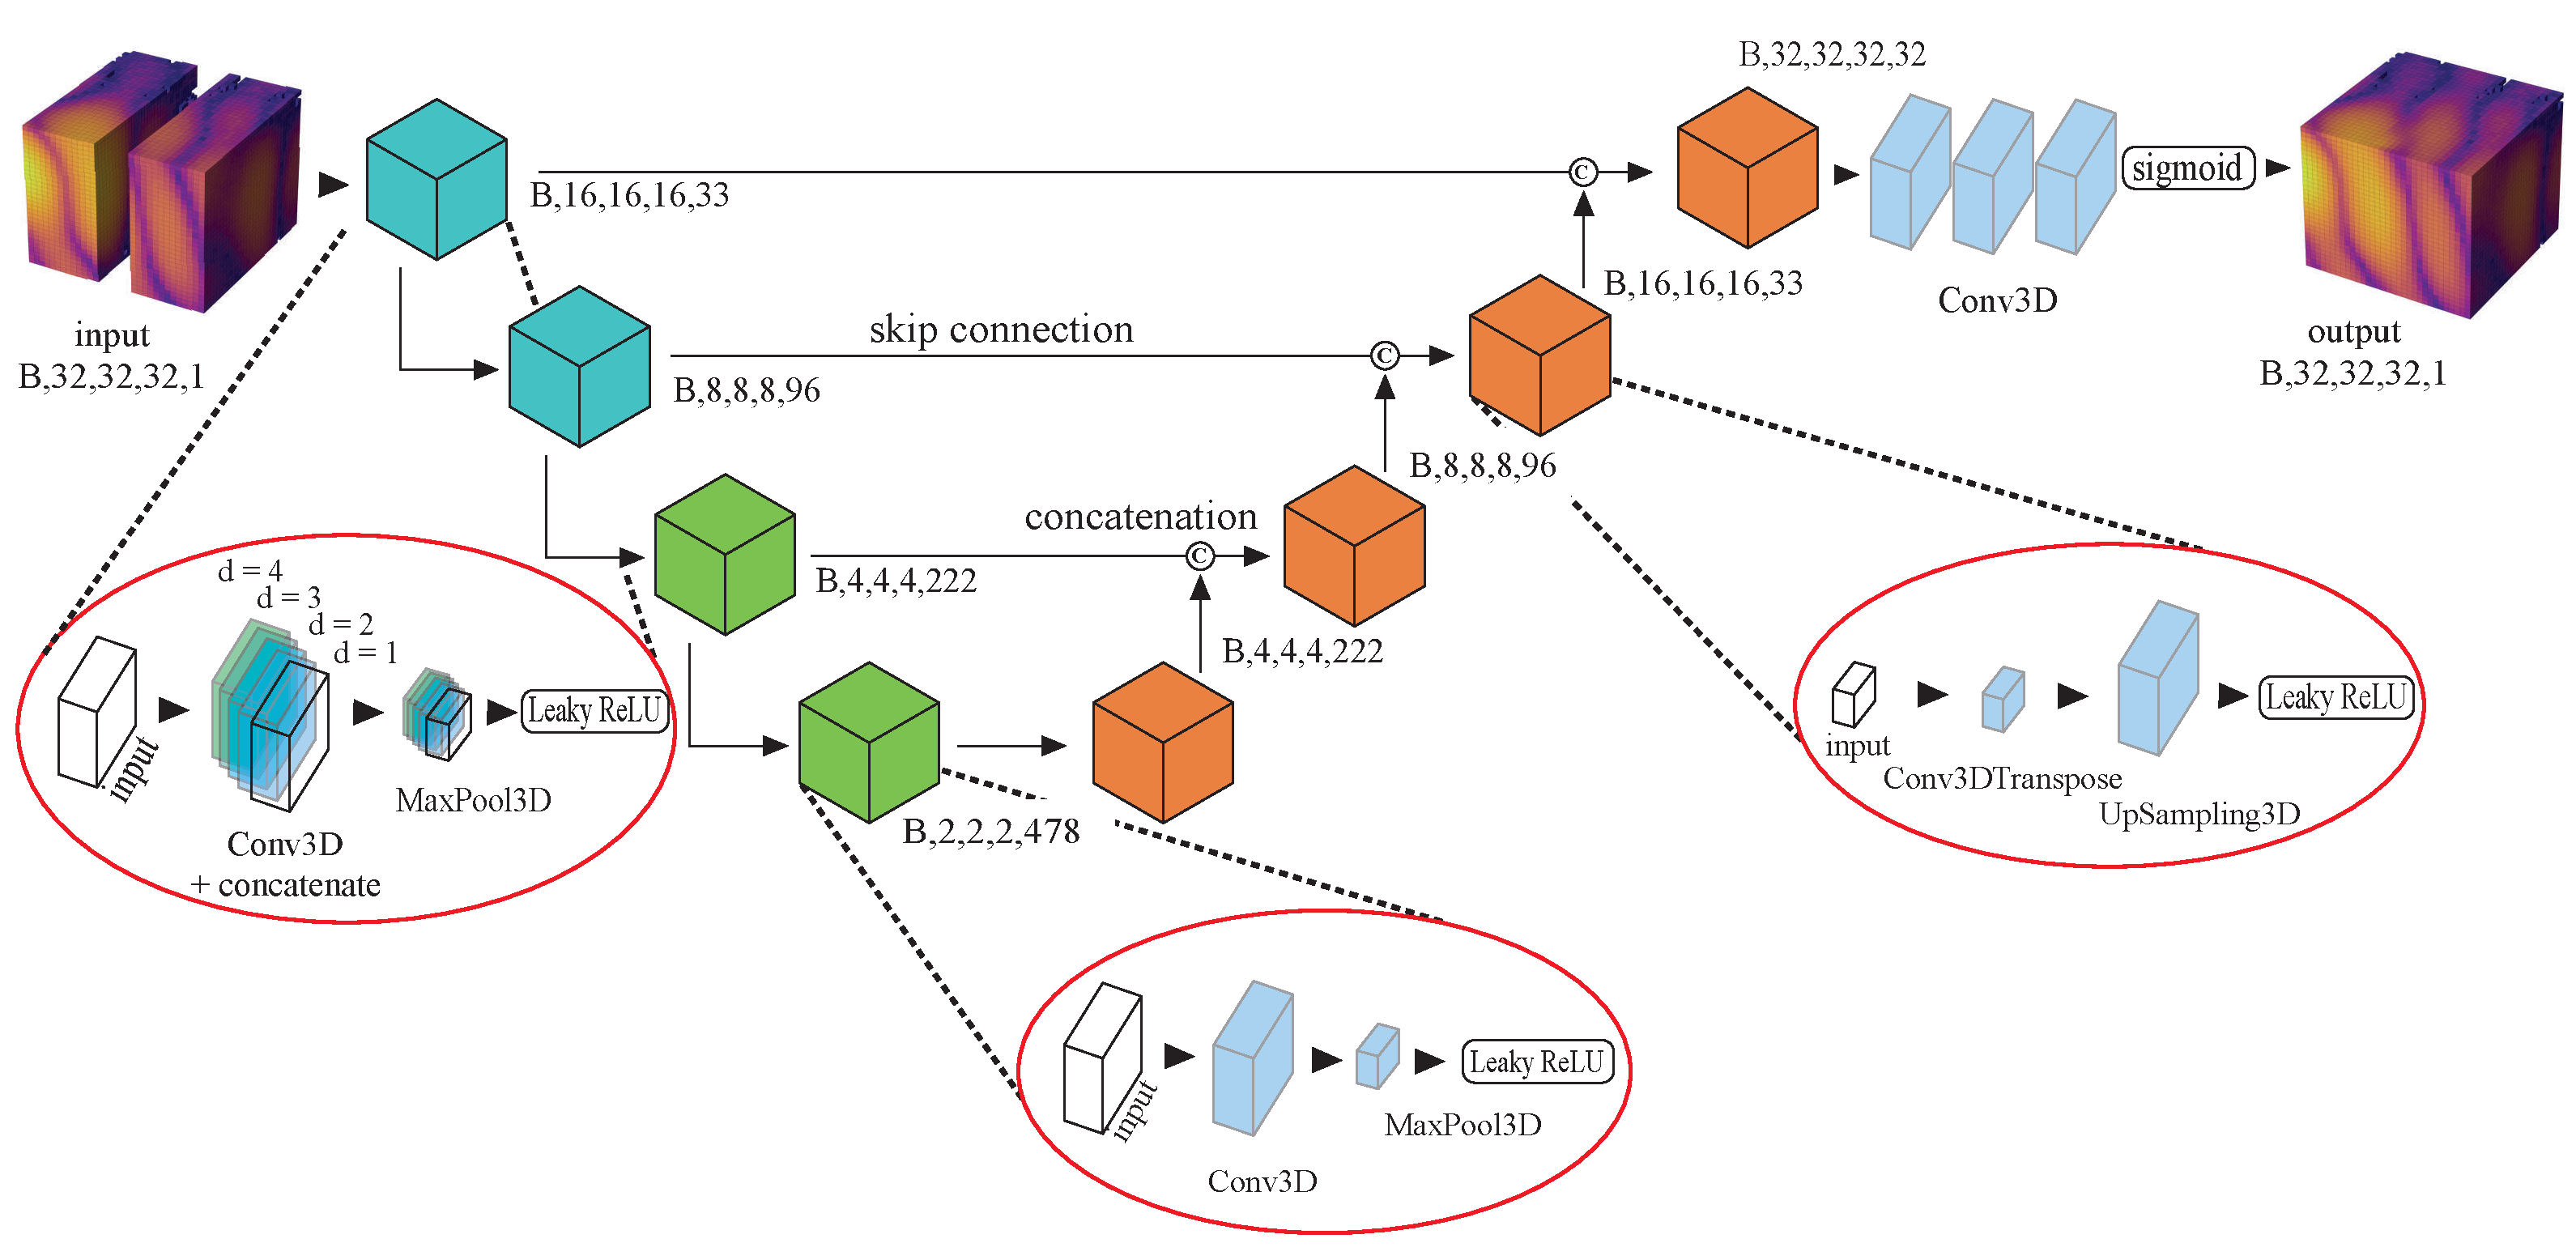
\includegraphics[width=\textwidth]{figures/Inpainting/Architecture_compressed.pdf}
    \caption{\textbf{Schematic of the 3D model architecture} The model uses a modified U-Net structure. 
    In the first two encoder blocks (highlighted by the left red circle), dilated convolutions are applied where the 
    original input is concatenated with its convolutions at various dilation rates (\textit{d = 4,3,2,1}) prior 
    to the MaxPooling operation. The input consists of small gap-affected portions, grouped into batches
     of 32 (B). These portions (top left) are progressively processed by the encoder until they are reduced to a 
     $ 2\times2\times2$ pixel-size feature map. In the decoder, each building block (represented as orange cubes) receives 
     as input the concatenation of the output from the previous block and the matching output from the encoder block 
     of the same size. The final result (top right) is a batch of inpainted versions of the input portions.}

    \label{fig:architecture3d}
\end{figure}

\section{Results in detector space}\label{sec:res_rec}

In this section we will present the results of our DL model on both simulated and experimental diffraction patterns. In
the next section we will move instead to the results in real space, therefore focusing more on the reduction of the artifacts 
in the reconstructed objects.\\

Once completed the training of the model we have first tested it on portions taken from the test dataset. It is possible
to qualitatively observe that the model works equally well for both simulated and experimental data (see Figs. \ref{fig:pred_portions_sim}
- \ref{fig:pred_portions_exp}). From a first visual assessment we can also confirm that low noise regions with larger features
are better restored than others as previously stated in Sec. \ref{sec:performances}. Another curious effect that we can observe, 
is the ``smoothening'' of features around noisy areas (see first column in Fig. \ref{fig:pred_portions_sim} and last column in Fig.
- \ref{fig:pred_portions_exp}). In fact, the ``grainy'' aspect of these regions is caused by Poisson noise which cannot
be predicted by the DL model as it is uncorrelated. In those regions the DL performs therefore a sort of average that 
``smoothens'' the features and acts like a denoiser. This effect has been already studied in the literature and exploited 
for denoising applications like the Noise2Void model \cite{Noise2Void}.

\begin{figure}[h]
    \centering
    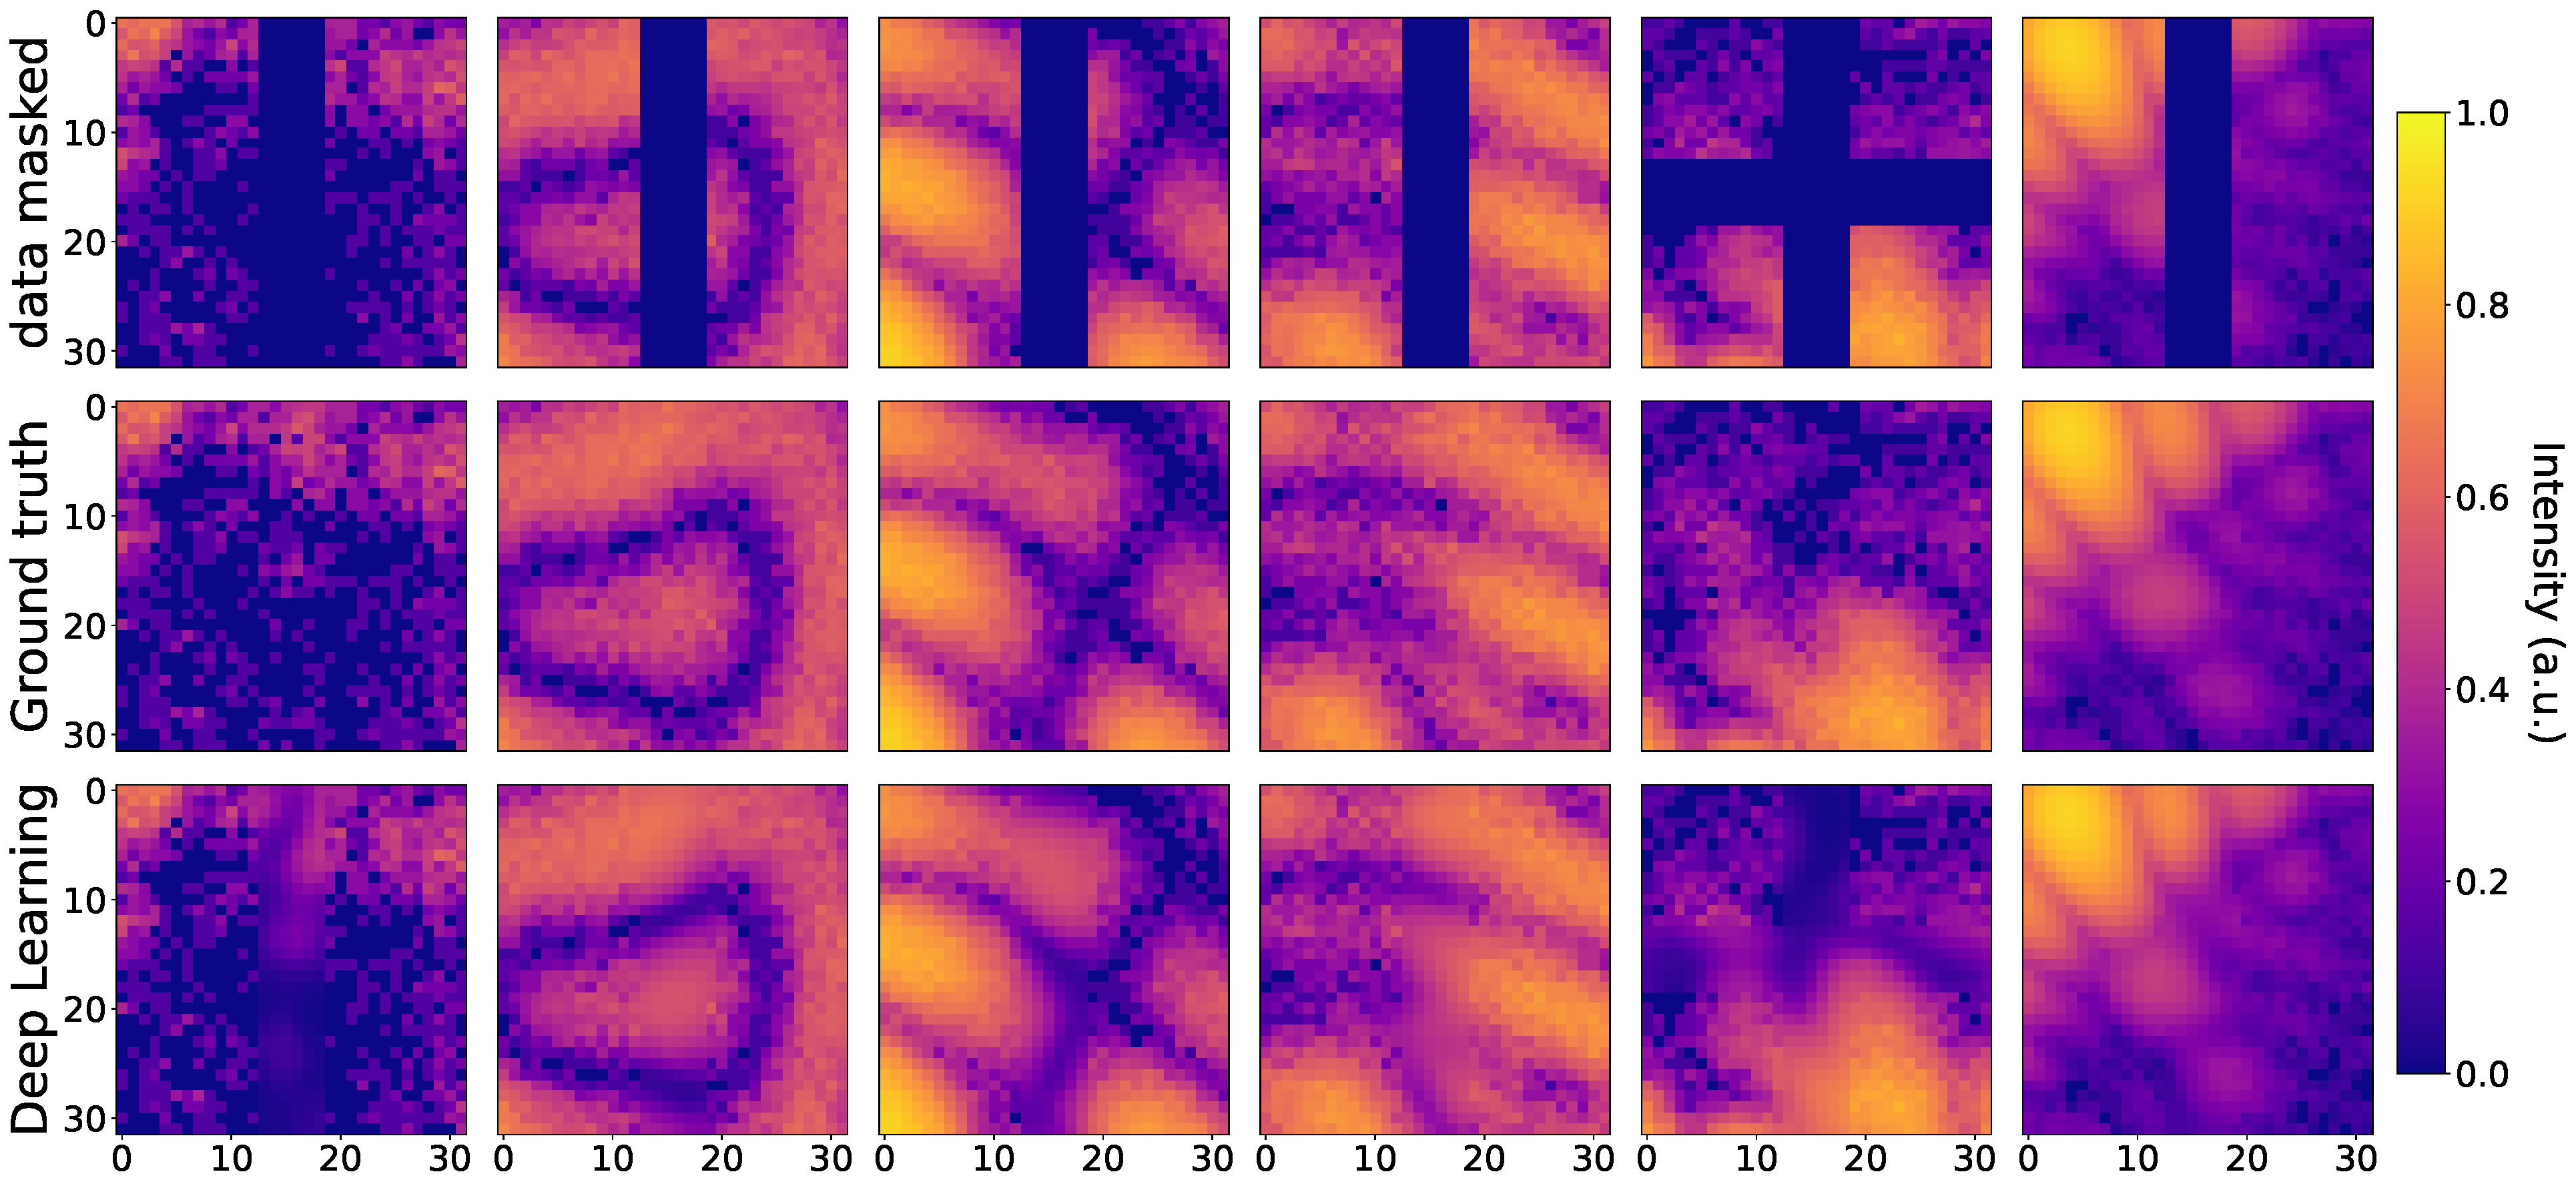
\includegraphics[width=\textwidth]{figures/Inpainting/prediction_small_simulated.pdf}
    \caption{\textbf{Results on portions of test simulated data}. Central slices of portions taken from the simulated test
    dataset. Masked input with 6 pixel-wide gap in the first row, corresponding ground truth and DL inpainted in second and third
    row respectively.}
    \label{fig:pred_portions_sim}
\end{figure}

\begin{figure}[h]
    \centering
    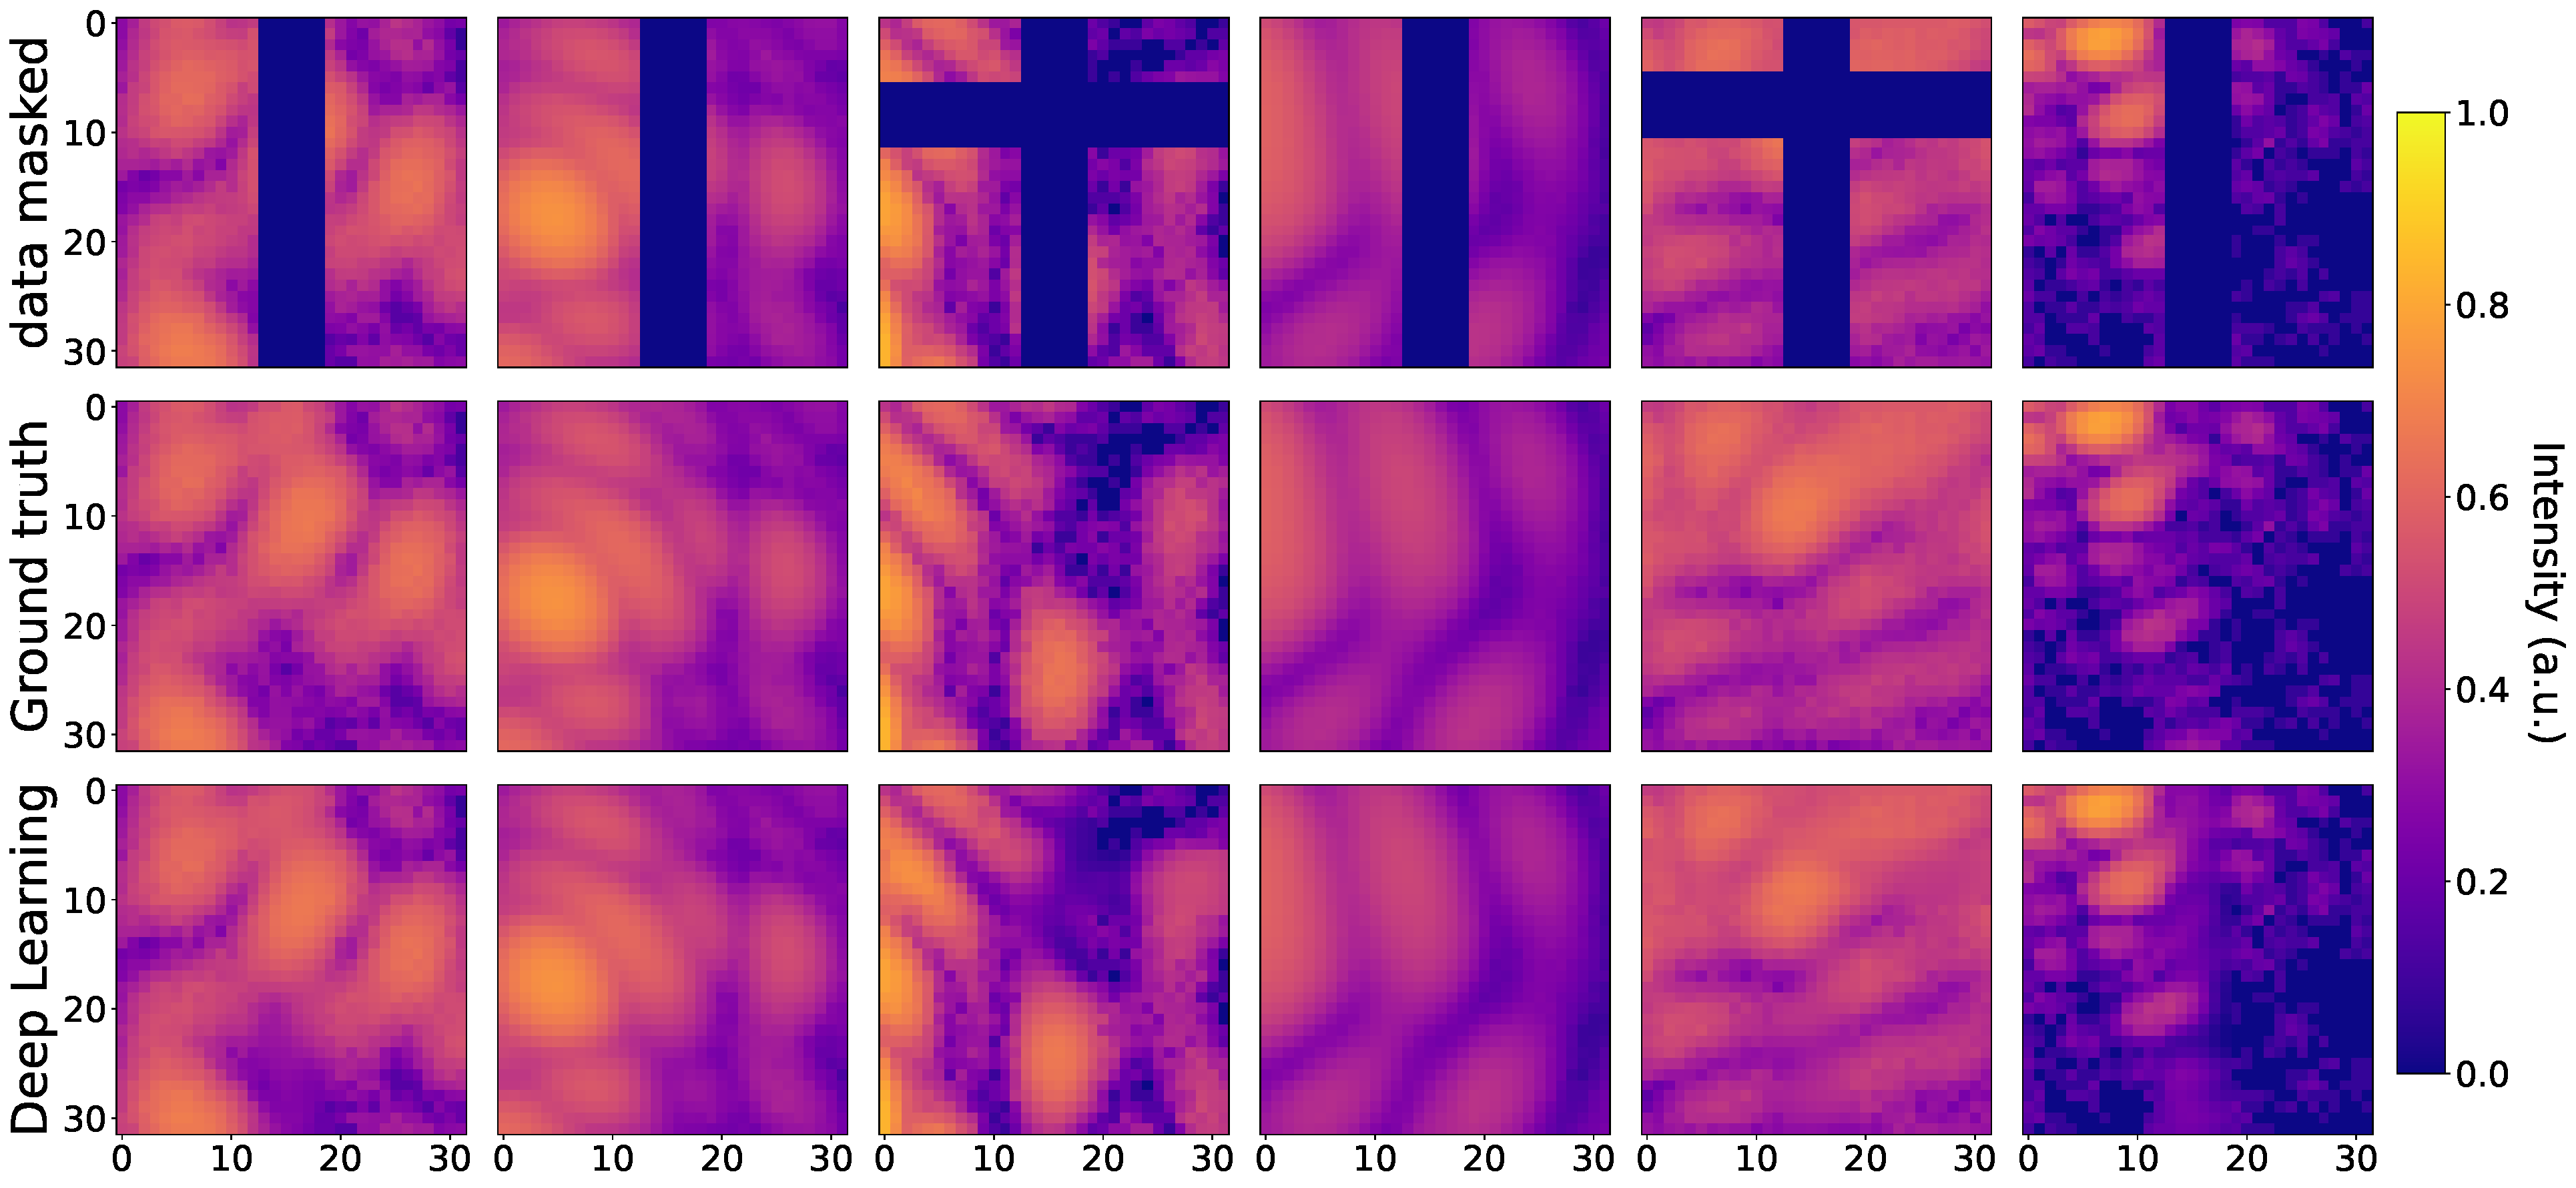
\includegraphics[width=\textwidth]{figures/Inpainting/prediction_small_experiment.pdf}
    \caption{\textbf{Results on portions of test experimental data}. Central slices of portions taken from the experimental test
    dataset. Masked input with 6 pixel-wide gap in the first row, corresponding ground truth and DL inpainted in second and third
    row respectively.}
    \label{fig:pred_portions_exp}
\end{figure}

\subsection{Full gap inpainting}\label{sec:full_gap}

For the inpainting of a gap inside a full 3D BCDI pattern it is sufficient to apply repeatedly the DL model on sub-volumes 
cropped such that the gap plane lies vertical in the center of the array perpendicularly to the third dimension. Each sub-
volume needs to be preprocessed exactly in the same way described above, i.e. transformed into logarithmic scale and 
normalized between 0 and 1. Moreover, it is advised to apply a mask on the gap, to match exactly the gap width the model
has been trained with. 
One can then proceed along the gap moving forward one pixel at the time, compute the inpainted gap and average the prediction
over the overlapping pixels with the previous predictions. By doing this, potential errors are averaged out and the accuracy
of the prediction is maximized. However, for large datasets this can be time-consuming. For example, for a $128\times128\times128$ pixel-size
diffraction pattern with a cross-shaped gap the time needed to compute the full inpainting amounts to 11 minutes (using a 
NVIDIA Tesla V100-SXM2 GPU with 32GB RAM). However, it is possible to increase the step size to significantly reduce the computing
time without affecting excessively the accuracy (see Fig.\ref{fig:skip_figure}). We have proven that the amount of time for the full inpainting follows a power 
law (see Fig. \ref{fig:skip_case}a) and the accuracy starts dropping significantly for more than 5 pixels skipped at the time
(see Fig. \ref{fig:skip_case}b).  

\begin{figure}[h]
    \centering
    \begin{subfigure}{0.45\textwidth} % Adjust width as needed
        \centering
        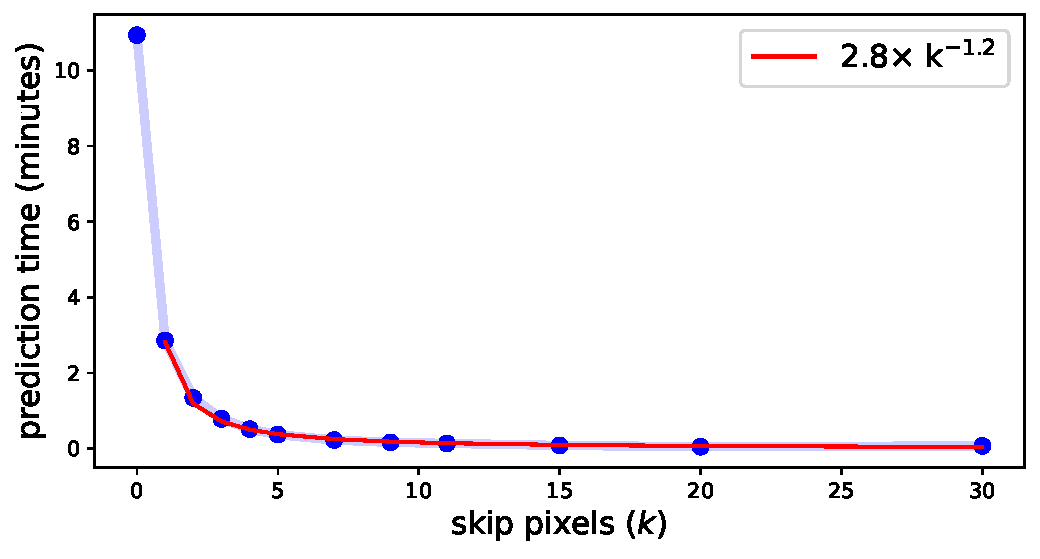
\includegraphics[width=\linewidth]{figures/Inpainting/skip_pixels_time.pdf}
        \caption{\textbf{(a)}}
    \end{subfigure}
    \hfill
    \begin{subfigure}{0.45\textwidth}
        \centering
        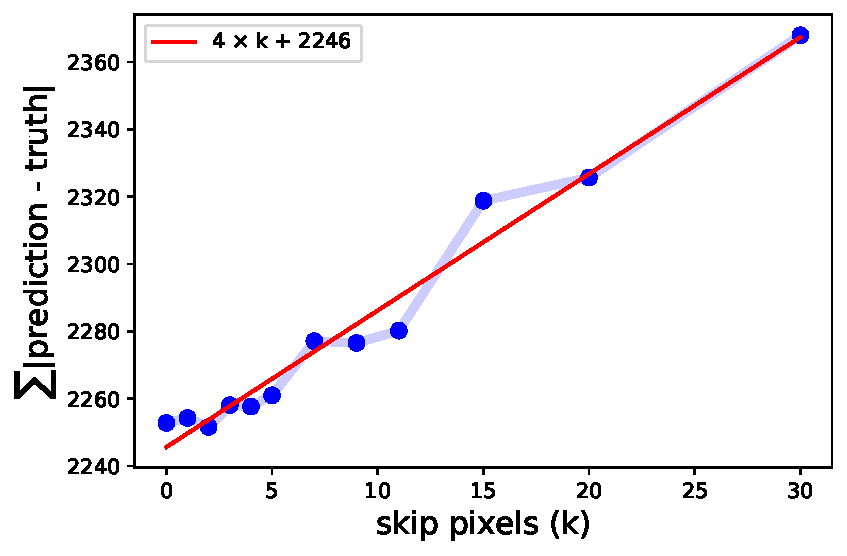
\includegraphics[width=\linewidth]{figures/Inpainting/skip_error.pdf}
        \caption{\textbf{(b)}}
    \end{subfigure}
    \caption{\textbf{(a)} Full inpainting time for a 6 pixel-wide cross-shaped gap on a  $128\times128\times128$ pixel-size
    diffraction pattern as function of the amount of pixels skipped between patch DL predictions along the gap.
    \textbf{(b)} Sum of the absolute errors as function of the skipped pixels. }
    \label{fig:skip_case}
\end{figure}

\begin{figure}[h]
    \centering
    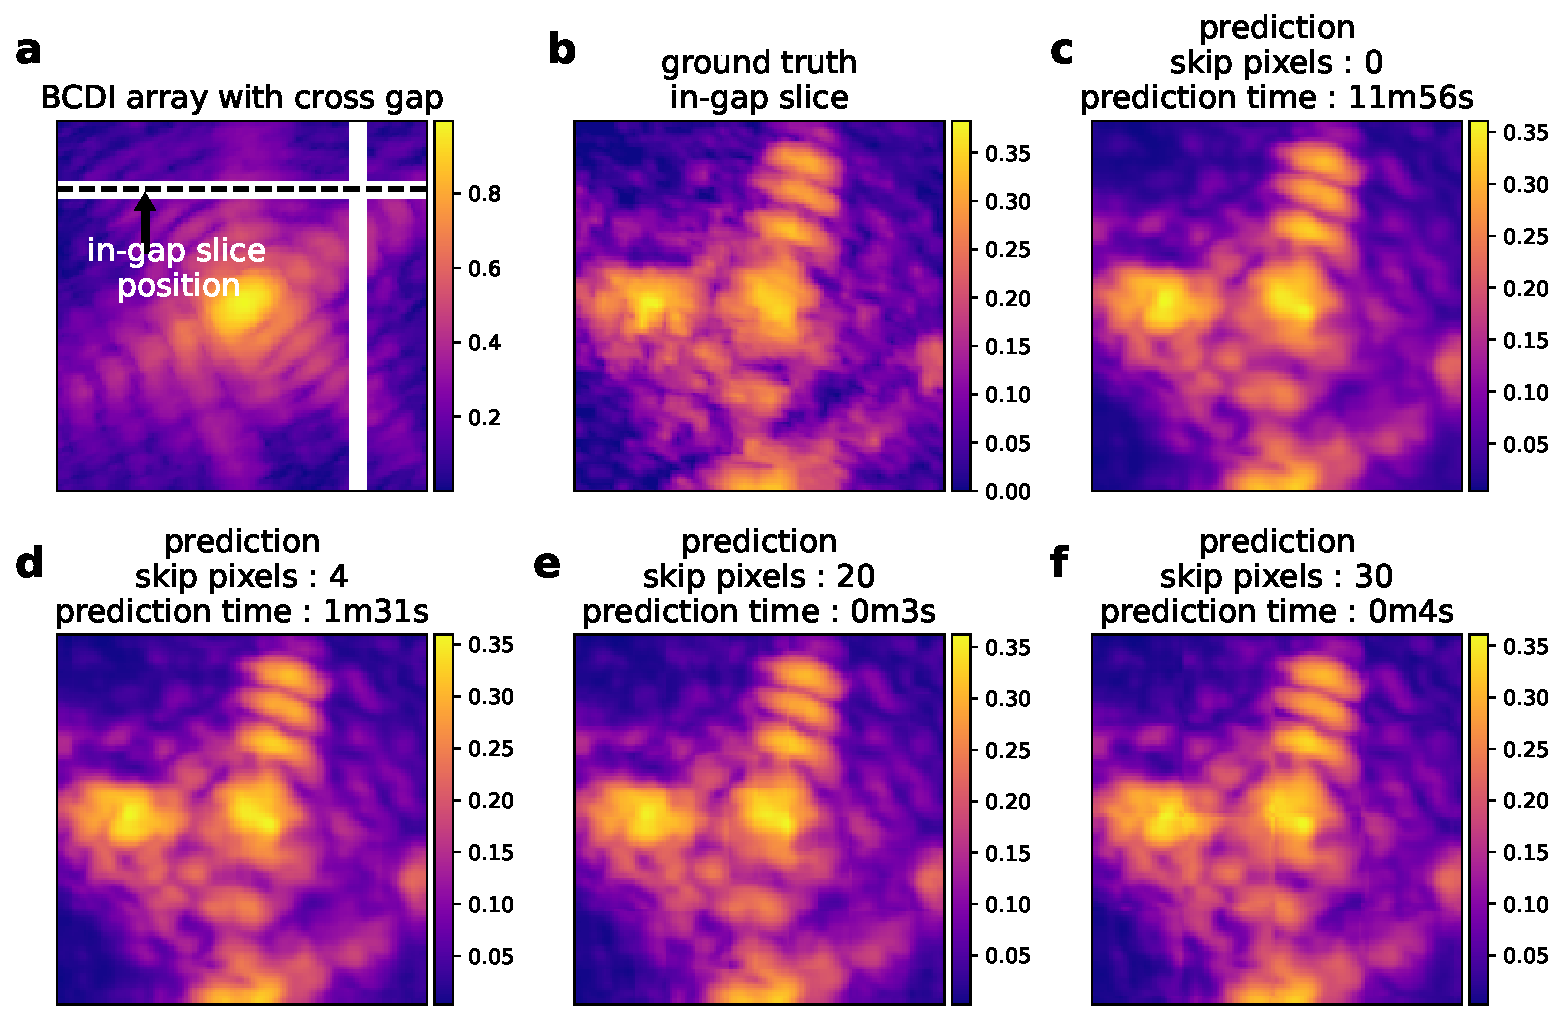
\includegraphics[width=\textwidth]{figures/Inpainting/Skip_pixels_ingap_slice.pdf}
    \caption{Full inpainting of an experimental BCDI pattern for different amounts of skipped pixels. \textbf{a}
    slice of the diffraction pattern perpendicular to the gap plane.\textbf{b} Ground truth intensity inside the gap.
    \textbf{c-d-e-f} In-gap prediction with 0, 4, 20 and 30 skipped pixels respectively, with corresponding 
    execution time. Skipping 4 pixels is a good trade off between time and accuracy.}
    \label{fig:skip_figure}
\end{figure}

\section{Performances assessment}\label{sec:performances}

In order to assess the performances of our DL model with respect to other inpainting methods, we tested it against 
conventional interpolation methods. Specifically, we have taken an experimental BCDI pattern with a 6 pixel-wide 
cross-shaped gap and compared the inpainting results of our DL model with (i) linear interpolation (ii) cubic interpolation 
(iii) nearest-neighbor interpolation. These techniques allow for a quick estimation of the intensity distribution 
inside the gaps but fail to recover fine features (see Figs. \ref{fig:interp}). In particular, we can notice 
in the \textit{in-gap slice} (Fig. \ref{fig:interp}a) that linear interpolation for instance doesn't retrieve correctly 
the space curvature of the fringes while nearest neighbor and cubic interpolations show artifacts in correspondence 
of the perpendicular gap. When considering the central slice perpendicular to the gap planes (along the rocking curve
dimension) we can notice even more how the DL model outperforms conventional interpolations (Fig. \ref{fig:interp}b).
 

\begin{figure}[ht]
    \centering
    \begin{subfigure}{0.47\textwidth} 
        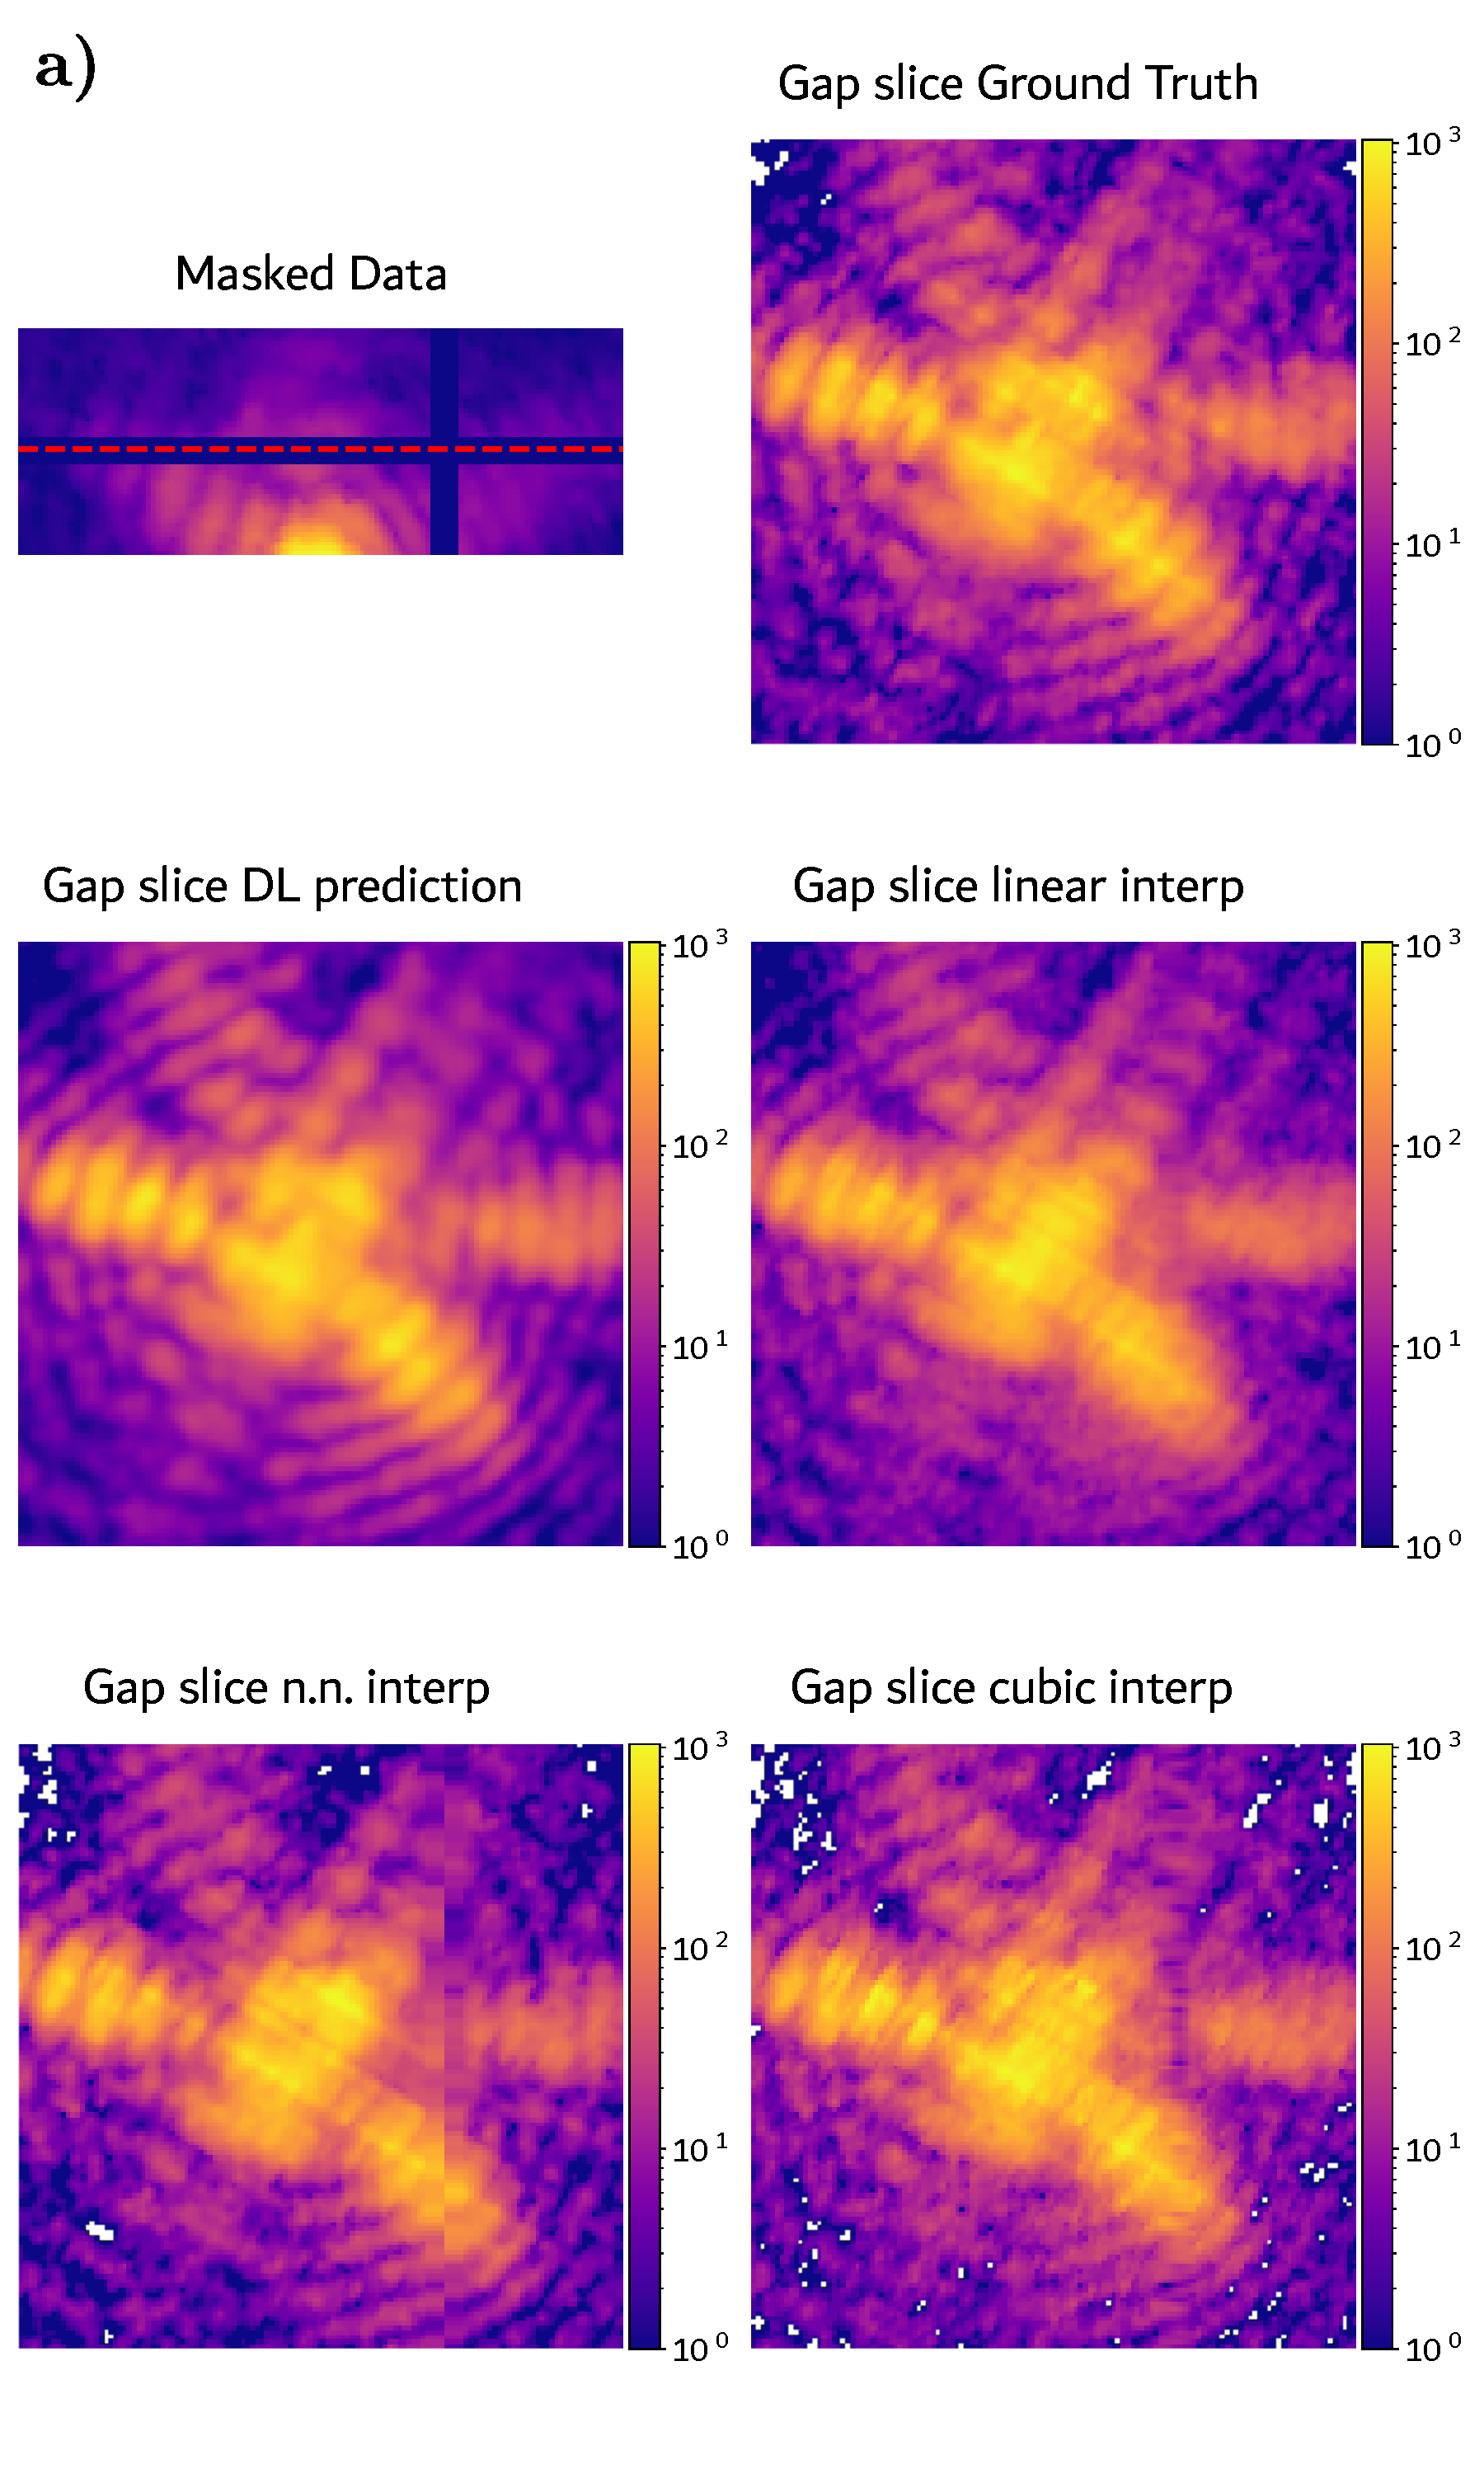
\includegraphics[width=\linewidth]{figures/Inpainting/newfig3_suppl.pdf}
        \caption{\textbf{(a)}}
    \end{subfigure}
    \hfill
    \begin{subfigure}{0.47\textwidth}
        \centering
        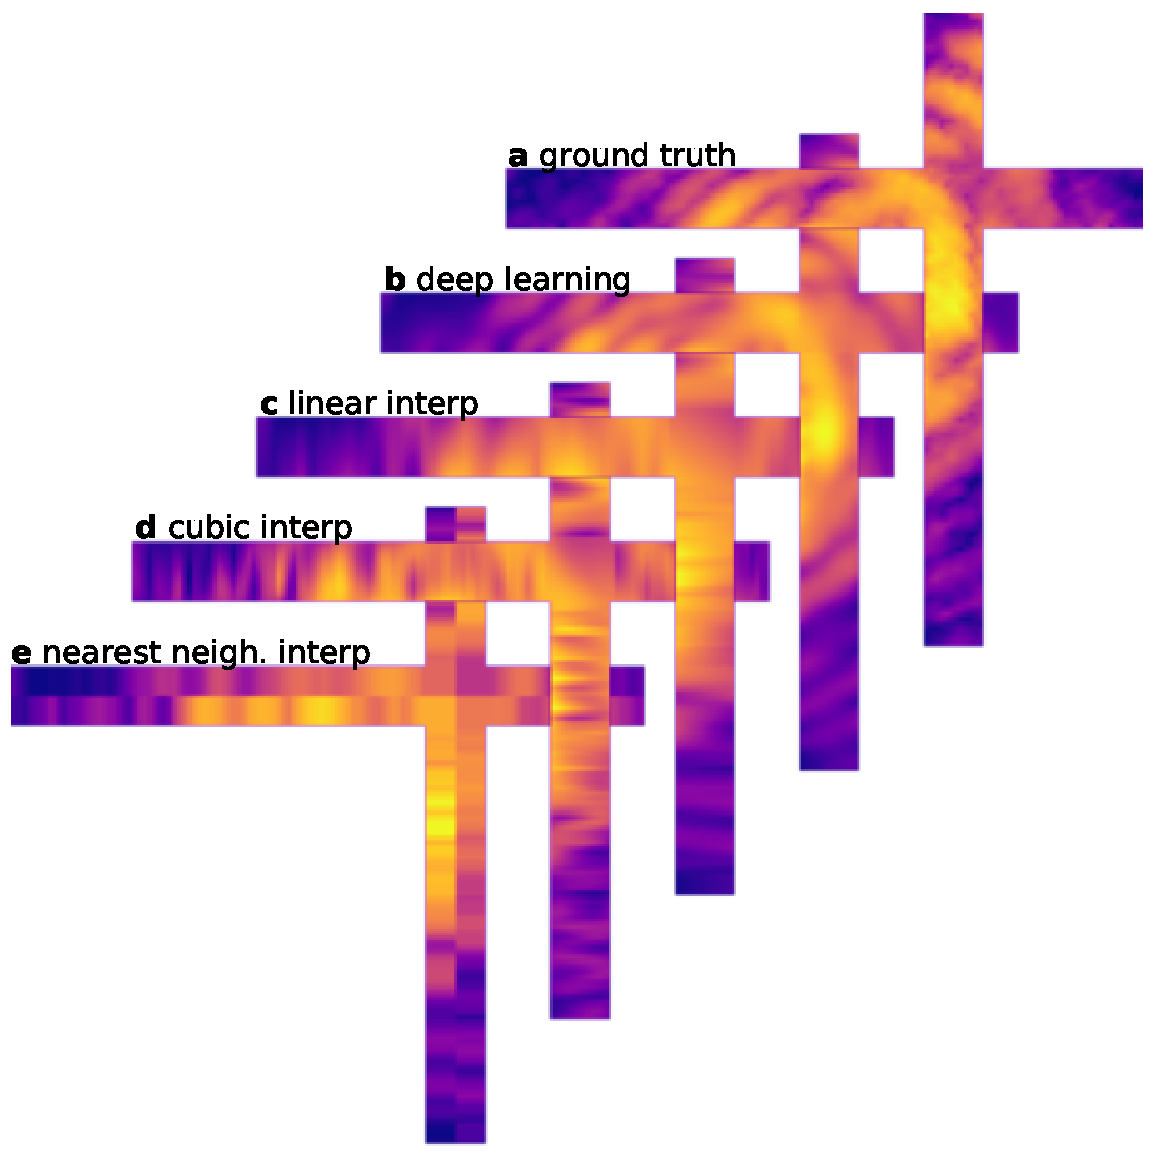
\includegraphics[width=\linewidth]{figures/Inpainting/cross_interp.pdf}
        \caption{\textbf{(b)}}
    \end{subfigure}
    \caption{}
    \label{fig:interp}
\end{figure}


Similarly to the 2D case above, we have also evaluated the performances of the model against the amount of intensity 
inside the sub-volume and against the oversampling ratio. We repeated the test for different gap widths, namely 3,6,9,12 
pixel-wide, using vertical gaps placed in the center of each portion. 
For the first performance assessment we have considered a full simulated $128\times128\times128$ pixel-size BCDI pattern
and randomly cropped out of it 1000 portions. We have then applied a vertical gap in the center of each portion for different 
gap sizes and then computed the prediction with the corresponding DL model. The intensity (in pixel counts) inside each sub-
volume was then summed and the obtained values for the 1000 samples were binned into 20 classes for better visualization. 
The accuracy scores, calculated with the PCC, were then averaged inside each bin class. The results are displayed in Fig. 
\ref{fig:acc_int_3D}. As expected from what discussed above for the 2D case, better accuracy scores are obtained for portions
containing larger amount of signals, where noise levels are lower and the features of the diffraction pattern are more 
visible. Moreover, the plot logically shows that smaller gaps are generally better recovered, but it is worth noticing
that the accuracy spread across different gap sizes widens for noisy portions and narrows down as the amount of signal 
increases. These trends suggest that DL models are overall robust to different gap sizes especially for high intensity regions, 
which are eventually the most important ones as they contribute the most during to the reconstruction. 

\begin{figure}[ht]
    \centering
    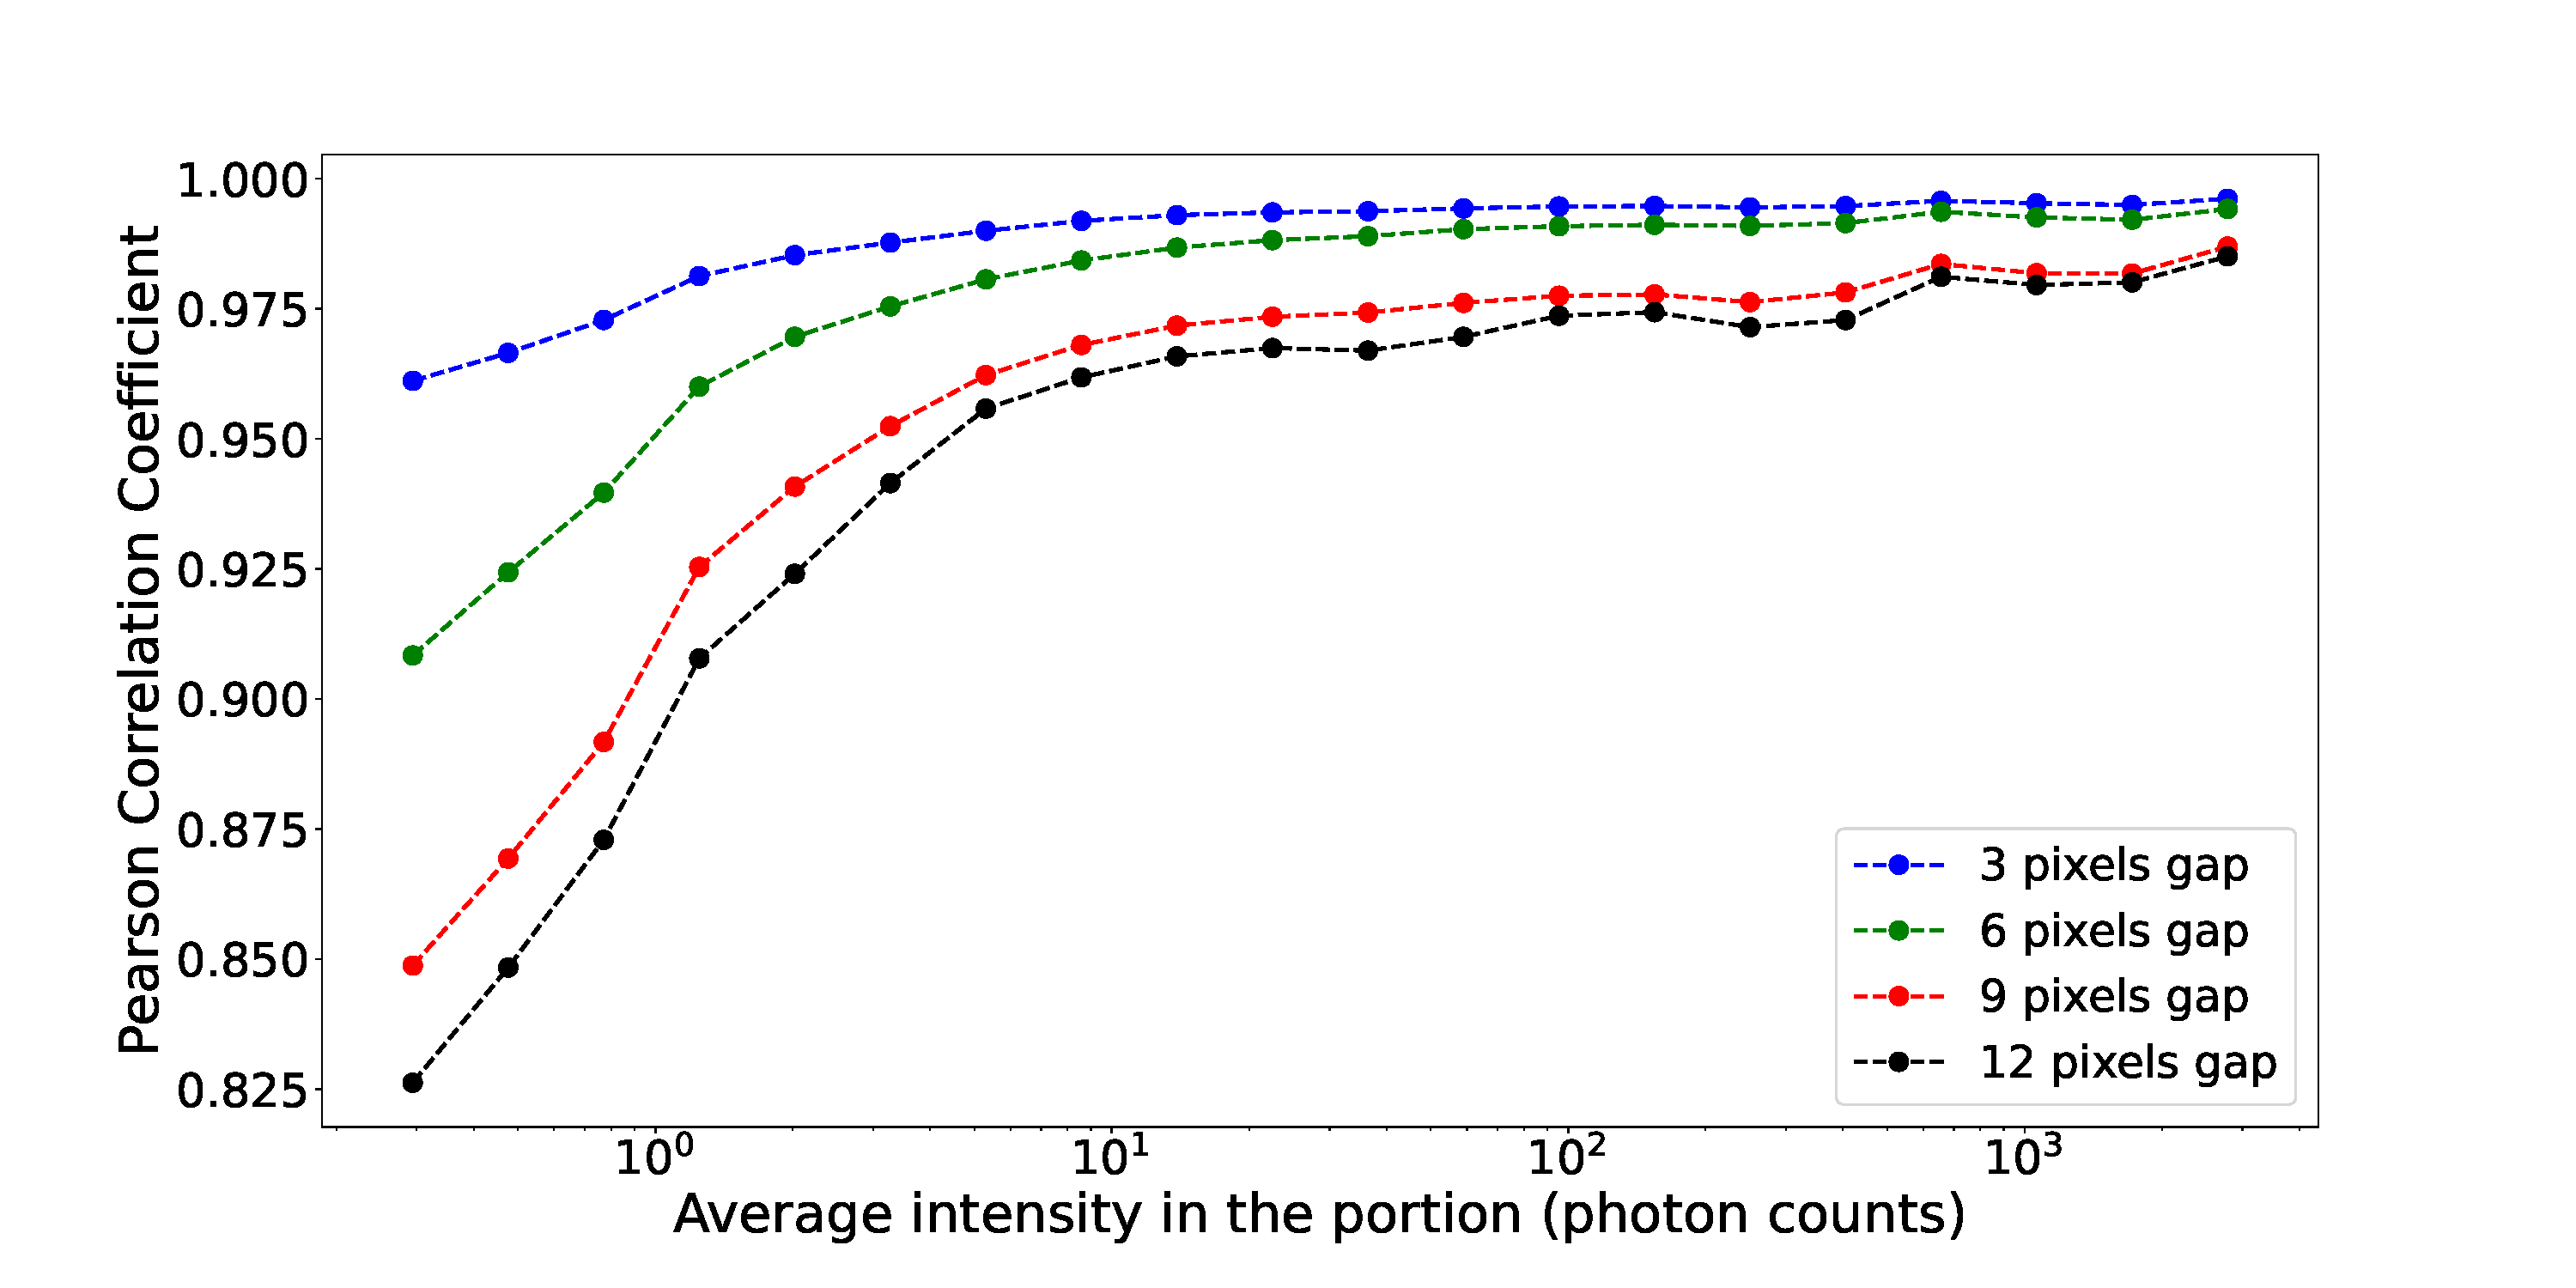
\includegraphics[width=\textwidth]{figures/Inpainting/1D_Acc_Intensity.pdf}
    \caption{Accuracy scores (PCC) of the DL patching model }
    \label{fig:acc_int_3D}
\end{figure}

The last test concerns the study of the accuracy for different oversampling ratios. As anticipated above for the 2D case, 
to carry out properly this evaluation, one should consider the same diffraction pattern extending to the same equivalent
$Q$-space value for each oversampling ratio. This in practice is done reducing increasing the $dq$ per pixel as decreasing
the oversampling ratio, resulting in a smaller size of the overall BCDI pattern. In our particular case we have simulated
the same BCDI pattern for oversampling ratios spanning from 2 to 7. For each oversampling ratio, a vertical gap
mask was applied to the whole BCDI array and the DL prediction was calculated with no-skip pixel (see Sec. \ref{sec:full_gap}).
The gap was then shifted laterally and this procedure was repeated until the whole BCDI array was predicted using our
model, thus leading to a full BCDI predicted image. The PCC was then calculated using the whole BCDI array for 
different oversampling ratios and model gap sizes. The results are displayed in Fig. \ref{fig:acc_ovs_3D}. As expected,
the predictions are more accurate for large oversampling ratios and small gap sizes (i.e., large oscillation periods 
relative to the gap width). 

\begin{figure}[ht]
    \centering
    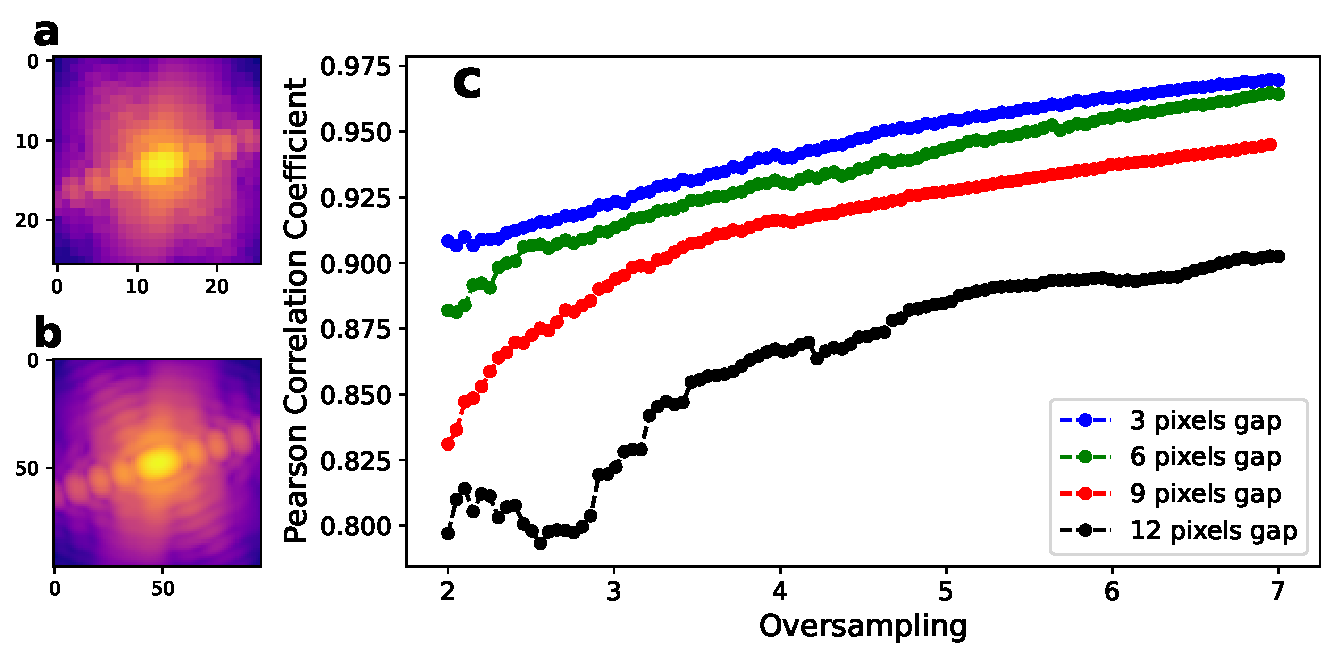
\includegraphics[width=\textwidth]{figures/Inpainting/accuracy_oversampling.pdf}
    \caption{Accuracy scores (PCC) of the DL patching model against the oversampling ratio. }
    \label{fig:acc_ovs_3D}
\end{figure}

\section{Results in real space}\label{sec:res_real}

In this section we will discuss the effects of DL inpainting on the reconstructed objects for both simulated and experimental 
data. In particular, for what concerns the simulated data we will proceed starting from the reconstruction of an experimental 
diffraction pattern subsequently modified to better show the artifacts produced by the gap and their reduction thanks to 
the DL model. The diffraction pattern is 



As we have said in the beginning of the chapter, the typical signature of a gap-affected diffraction pattern is the
presence of oscillatory artifacts in both modulus and phase  



\section{Fine-tuning}\label{sec:finetuning}

